% \chapter{Selection contributes to skewed X chromosome inactivation across human tissues}

% \section{Background}
% X chromosome inactivation (XCI) occurs in blastocysts during embryonic development. Under no external pressures, the process is assumed to be random and is established in about a dozen cells and all daughter cells will inherit the XCI status of these cells\cite{Takagi1975-es}. Skew in XCI has been widely observed in female mammals and is accepted to be common across individuals\cite{Shvetsova2019-re}. Selective pressures have been implicated in contributing to XCI skew, especially in the context of diseases such as cancer\cite{Brown1999-dc,Migeon1998-gc,Brooks2014-pz}. In addition, XCI skew was found to be heritable and correlated with age based on a twin study\cite{Zito2019-hu}. Recent work argued that observed XCI skew in the general female population is the result of expected randomness in early development\cite{Shvetsova2019-re}. 

% Here, we show that estimated XCI skew in a general female population in the GTEx dataset\cite{GTEx_Consortium2020-xx} is associated with genetic scores related to deleteriousness and proliferative potential. We hypothesize that differences in the fitness of maternal and paternal X chromosomes may contribute to skewed XCI across tissues into adulthood (Figure \ref{fig:fig4.1}a).  Furthermore, we perform a scan of common variants across the X chromosome to identify specific loci associated with overall XCI skew in these individuals.

% \begin{figure}[ht]
    \centering
    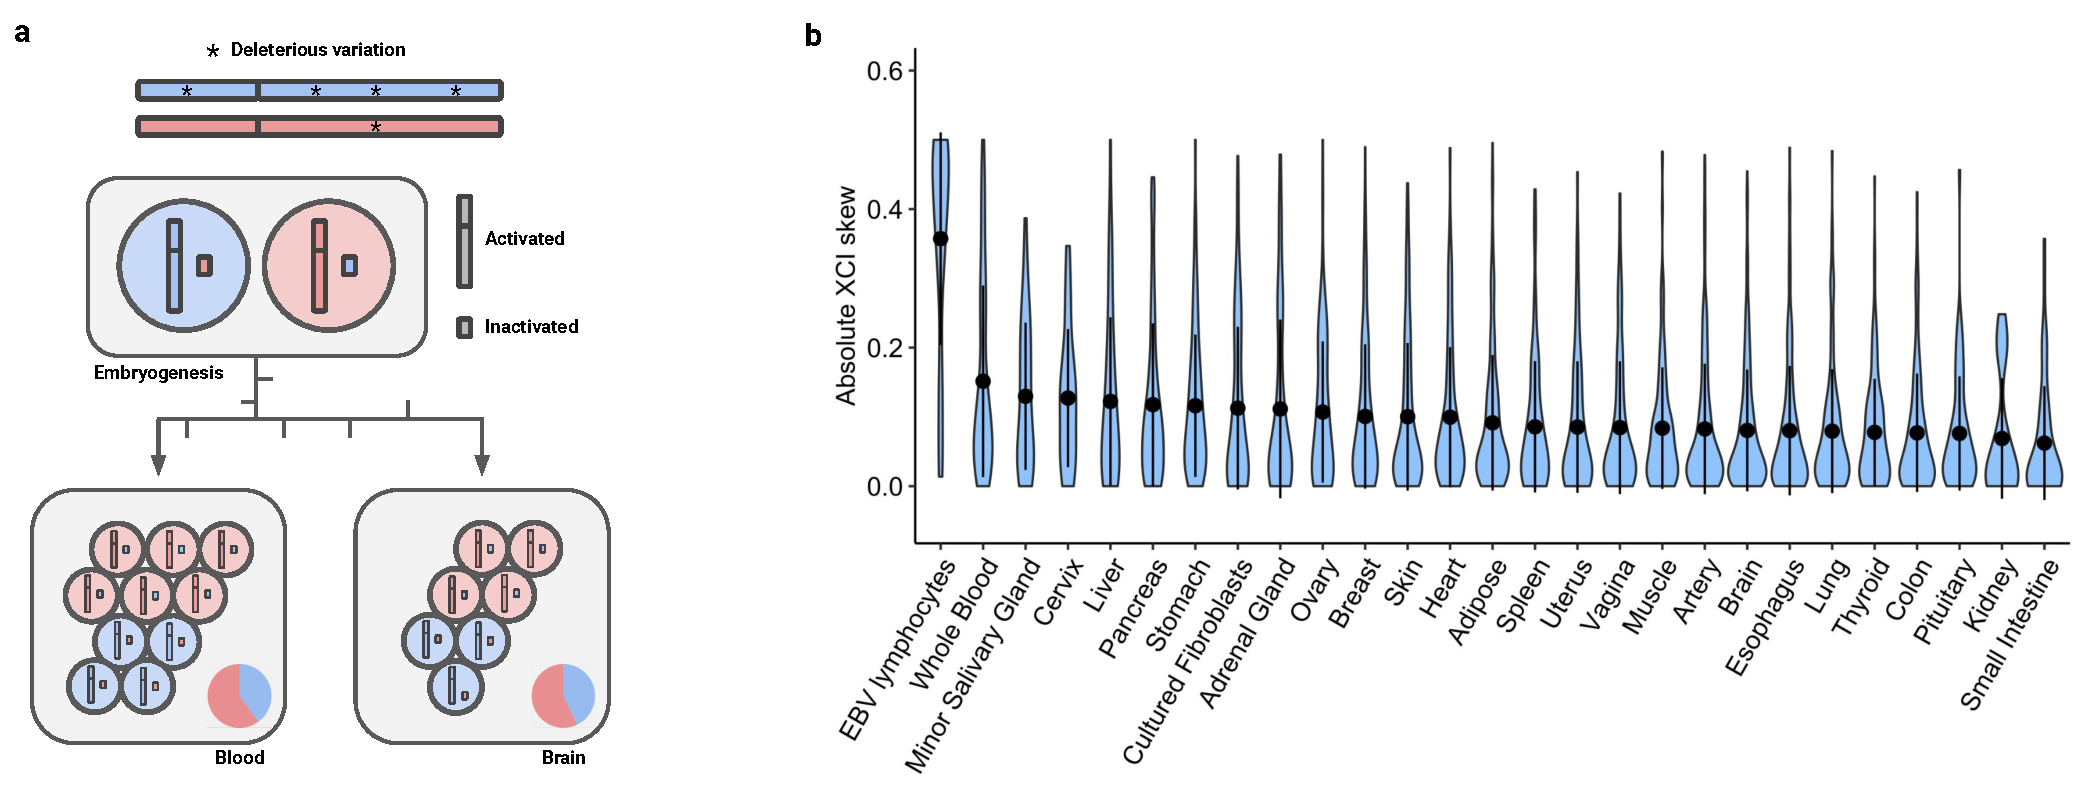
\includegraphics[width=\textwidth]{chapter4/Figures/Figure_1.pdf}
    \caption{
        Measuring XCI skew across tissues 
        \textbf{a}, Schematic overview of selection hypothesis. An individual inherits one haplotype (red) that is more fit than the other (blue) due to genetic variation. Given equal population sizes in embryonic development, we hypothesize that fitness differences will produce skewed populations in fully developed tissues.
        \textbf{b}, Violin plot of absolute XCI skew on the y-axis. Tissues are sorted by mean on the x-axis. Dots indicate mean of the absolute skew with vertical lines indicating one standard deviation.}
    \label{fig:fig4.1}
\end{figure}

% \section{Methods}
% \subsection{Transcriptomic and genetic data}

% The following data were processed and made available by the GTEx consortium \cite{GTEx_Consortium2020-xx}. GENCODE v26 and the GRCh38 human reference genome was used to process both WGS and RNA-seq data. RNA-seq data was aligned using STAR with WASP filtering. Allele-specific read counts at heterozygous sites were quantified with GATK ASEReadCounter. Genetic variants were called from whole genome sequencing data and phased with read-aware SHAPEIT2. All analyses were restricted to caucasian samples. 

% \subsection{Quantifying XCI skew}

% Allele-specific read counts were matched to haplotypes from the phased WGS data. Only heterozygous sites within fully inactivated genes reported by Carrel and Willard \cite{Carrel2005-zm} and Cotton et al \cite{Cotton2013-jl} were considered. Furthermore, we restricted to genes where no females were observed to escape inactivation in Cotten et al. LiftOver (https://genome.ucsc.edu/cgi-bin/hgLiftOver) was used to convert these reported gene windows from GRCh37 to GRCh38 positions. Moreover, we only considered variants that had at least 10 overlapping reads. XCI skew was calculated at each heterozygous site in the gene windows as the number of reads coming from haplotype 1 divided by the total number of reads at the site. The final XCI skew measurement for each sample was the median of these per-site observations. In addition, since haplotypes are not readily distinguishable as maternal or paternal, we also calculated the absolute XCI skew as the absolute deviation of this value from 0.5. 

% We also calculated skew in the same manner in autosomes. Specifically, if $m$ heterozygous sites were used to calculate XCI in a sample, we randomly selected $m$ heterozygous sites with at least 10 overlapping RNA-seq reads on the q-arm of each non-acrocentric autosome. We used these sites to calculate skew for each autosome. 

% \subsection{Genetic score association}

% Four scores were defined to measure genetic burden of X chromosome haplotypes in females. First, we considered the difference in average CADD score \cite{Rentzsch2019-pk} between the two haplotypes. A higher CADD score corresponds to an increased likelihood of deleteriousness. CADD Phred scores were retrieved using VEP \cite{McLaren2016-jd}. The CADD score associated with each alternate allele on each haplotype was averaged. The remaining scores were proportions of different types of mutations carried by a haplotype. We considered the proportion of alternate alleles, missense mutations, and synonymous mutations carried by a haplotype. This proportion is calculated as the count of the variant-type on one haplotype divided by the total number of these variants found across both haplotypes. Annotations indicating the coding consequence of variants were obtained using VEP.

% We associated these scores with XCI skew using a linear mixed model. Specifically, we used the lmer function from the lmerTest package \cite{Kuznetsova2017-jp} to fit the following model across all tissues, where the (1\textbar Grouping) notation indicates a random intercept for the specified grouping:
% \begin{equation}
% \text{H1 XCI Skew} \sim \text{H1 Burden + Age + (1\textbar Individual) + (1\textbar Tissue)}
% \end{equation}
% In this model, we include random intercepts for the individual and tissue of origin for each sample. The significance of these associations were determined using a one-sided t-test, under the assumption that increased burden will decrease skewing towards a haplotype.

% Blood-related polygenic scores were retrieved from PGS Catalog \cite{Lambert2021-iu}. We used scores for the following cell counts: platelet (PGS000186), red blood cell (PGS000187), basophil (PGS000163), neutrophil (PGS000182), eosinophil (PGS000165), monocyte (PGS000177), and lymphocyte (PGS000172) \cite{Vuckovic2020-gf}. GRCh38 positions of the variants used for these scores were retrieved from SNP Nexus \cite{Oscanoa2020-ac}. We calculated each polygenic score for both haplotypes and modeled the difference in scores as follows:
% \begin{equation}
% \text{H1 XCI Skew} \sim \text{(H1 PGS - H2 PGS) + Age + (1\textbar Individual) + (1\textbar Tissue)}
% \end{equation}
% The significance of these associations were determined by using a one-sided t-test, under the assumption that increased proliferative potential will increase skewing towards a haplotype. 

% Each of these tests were also performed for autosomes as controls with the following model:

% \begin{align}
% \begin{split}
% \text{H1 XCI Skew} \sim & \text{ (H1 PGS - H2 PGS) + Age +} \\
%                         & \text{ (1\textbar Individual) + (1\textbar Tissue) + (1\textbar Chromosome)}
% \end{split}
% \end{align}
% where “Chromosome” refers to the autosome used to calculate skew. A Bonferroni-corrected significance threshold of 0.05/8 was used for the 4 burden scores and 0.05/14 was used for the 7 blood-related polygenic scores. 

% \subsection{Identifying significant XCI loci}

% The phased X chromosome variants were filtered with PLINK 2 \cite{PLINK2}. SNPs were extracted with a minor allele frequency threshold of 0.01 and Hardy-Weinberg equilibrium p-value threshold of 1e-6. LD pruning was performed with a window size of 100 kilobases, step size of 5 variants, and $r^2$ threshold of 0.5. 

% These filtered variants were marginally tested in a linear mixed model to measure association with absolute XCI skew. We fit the following linear mixed model:
% \begin{equation}
% \text{Absolute XCI Skew} \sim \text{Heterozygous + Age + (1\textbar Individual) + (1\textbar Tissue)}
% \end{equation}
% where Heterozygous is 1 if the sample is heterozygous for the variant and 0 if the sample is homozygous. We modeled absolute skewing under the assumption that heterozygosity will lead to differences in fitness and consequently increased overall skewing. Given this assumption, we determined the significance of these associations using a one-sided t-test under this hypothesis. The resulting p-values were converted to q-values \cite{Storey2003-kx} and considered significant using a threshold corresponding to a 0.05 local false discovery rate.

% At the two significant loci, this linear mixed model was also used to determine the significance of the difference in skewing between homozygous samples and groups defined by the phasing of the variant in heterozygous individuals. For these associations, we fit the following model separately for individuals with the variant on H1 and on H2:
% \begin{equation}
% \text{H1 XCI Skew} \sim \text{Heterozygous + Age + (1\textbar Individual) + (1\textbar Tissue)}
% \end{equation}
% Since we do not assume the direction of individual variant effects on XCI skewing, we performed a two-sided t-test to determine significance of these associations. 

% \subsection{Associating XCI-linked genetics in males}

% To address the possibility that the burden and proliferation scores are capturing regulatory effects, such as downregulation of a haplotype rather than increased inactivation, we calculated these scores within males. Like in the female samples, we utilized variants outside of the fully inactivated genes used to calculate skew. Given that males have one X chromosome, we associated these scores with the expression of each gene on the X chromosome. We fit a model similar to those used for identifying expression quantitative trait loci. Specifically, we performed a linear regression within each tissue independently, correcting for the top 5 genetic principal components, PCR, and platform. We also corrected for PEER factors, \cite{Stegle2012-uf} using 15 for sample sizes less than 150 and adding an additional 15 factors for each 100 samples. The resulting p-values from the linear regression were converted to q-values \cite{Storey2003-kx} and considered significant at a local false discovery rate threshold of 0.05. 

% \section{Results}

% \subsection{Estimating XCI skew from RNA-seq data}

% We analyzed data generated by the GTEx consortium \cite{GTEx_Consortium2020-xx}, which included RNA-seq and phased whole genome sequencing data measured across 243 caucasian female samples and 472 caucasian male samples. We measured XCI skew in females as the difference in expression measured from each X chromosome in an RNA-seq experiment. Since XCI does not completely silence the entire X chromosome, we restricted our analysis to genes that have been previously observed to be fully inactivated \cite{Carrel2005-zm,Cotton2013-jl,Tukiainen2017-xm}. Read counts at heterozygous sites in these regions were assigned to haplotypes determined with phased whole genome sequencing data. The skew in RNA-seq reads was calculated at each site as the number of reads coming from one haplotype divided by the total number of reads. XCI skew for a sample was calculated as the median of these values. A median of 45 heterozygous sites were used for this calculation across the samples (Figure \ref{fig:supp_fig4.1}). We observed variability in XCI skew across tissues, with EBV-transformed lymphocytes exhibiting nearly complete skew in many samples (Figure \ref{fig:fig4.1}b).  Given this extreme skewing likely due to culture conditions, we removed these samples from downstream analyses. Furthermore, we observed correlation of XCI skew across the different tissues (Figure \ref{fig:supp_fig4.2}).

% \begin{figure}[ht]
    \centering
    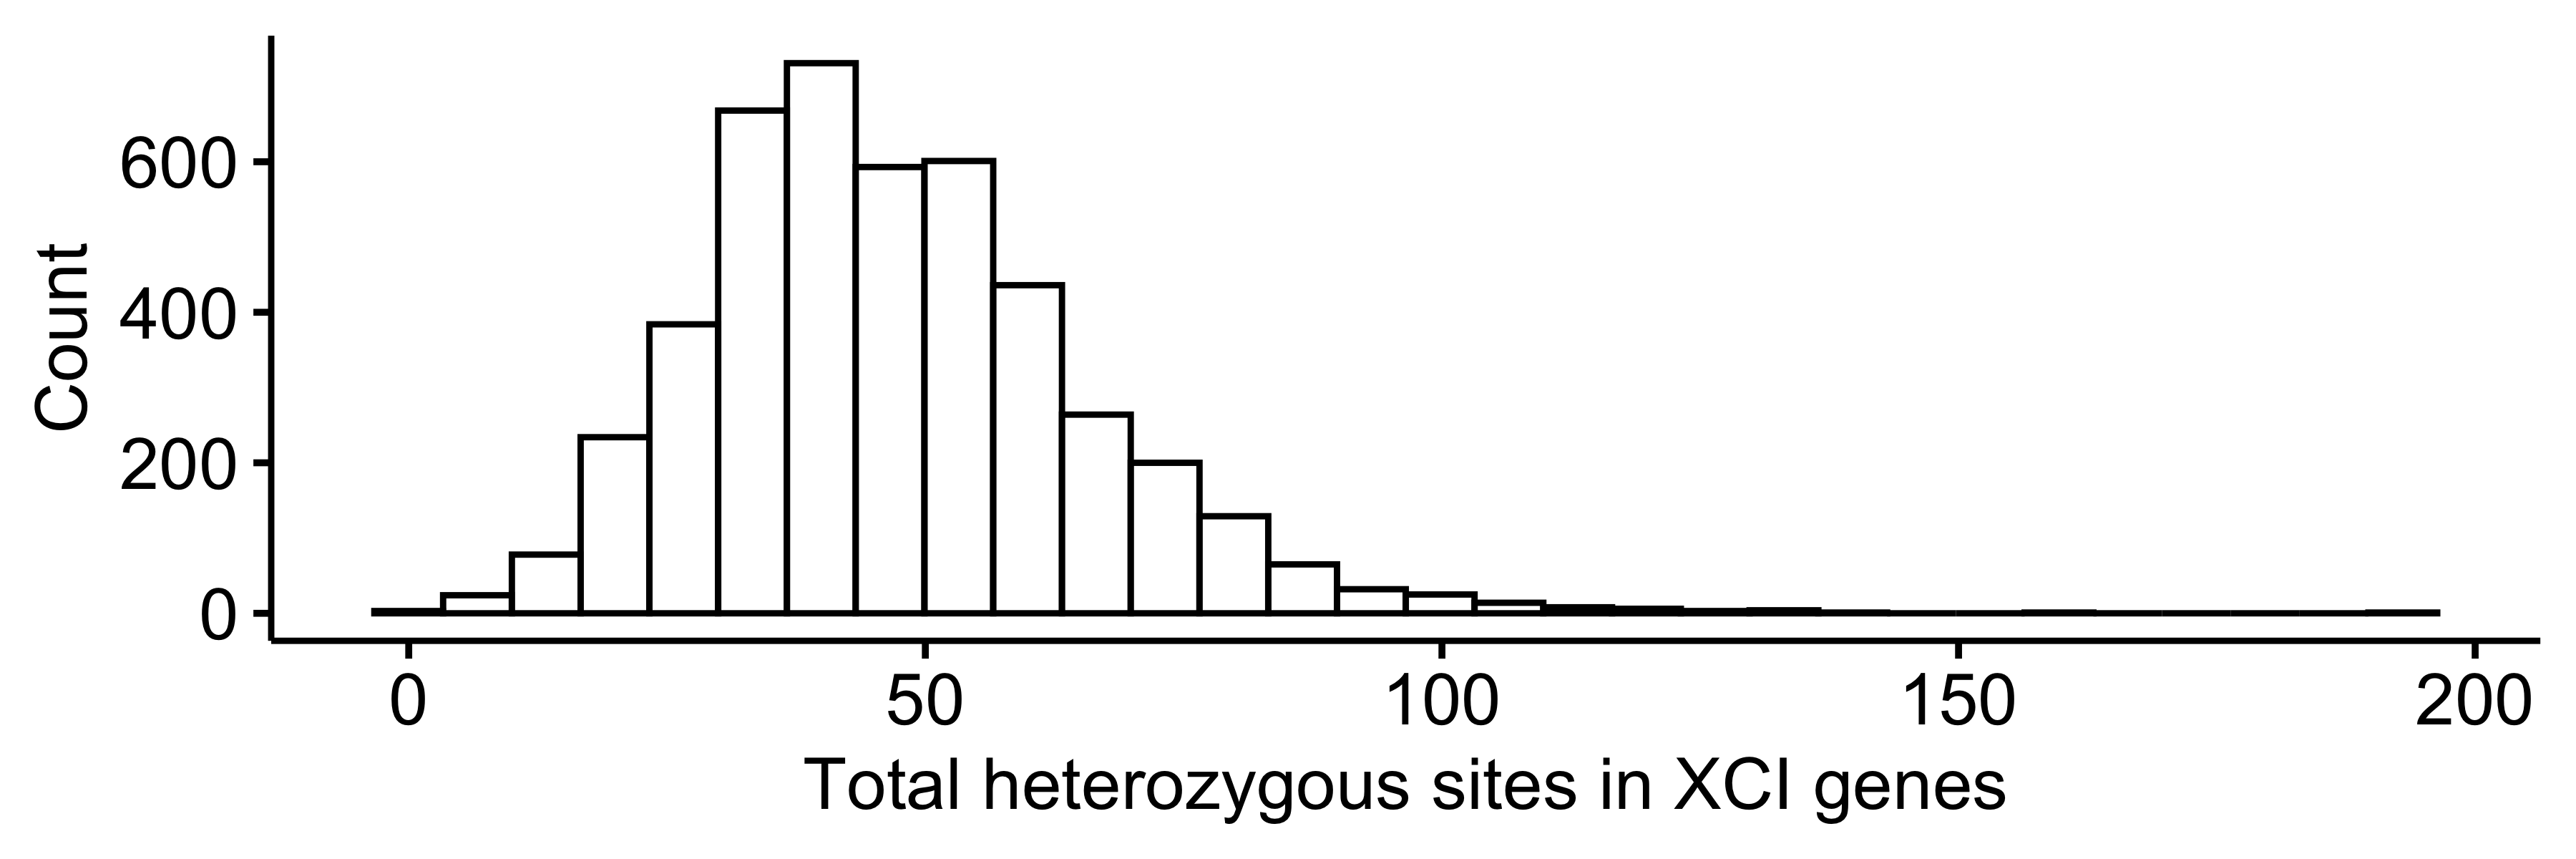
\includegraphics[width=0.75\textwidth]{chapter4/Figures/Supplementary_Figure_1.png}
    \caption{
        Histogram of number of heterozygous sites with coverage of 10 or more RNA-seq reads and within fully inactivated genes used to calculate XCI skew for each sample. We observed a mean of 46.805 and median of 45 variants used to calculate skew (the median of per-site skew). 
    }
    \label{fig:supp_fig4.1}
\end{figure}
% \begin{figure}[ht!]
    \centering
    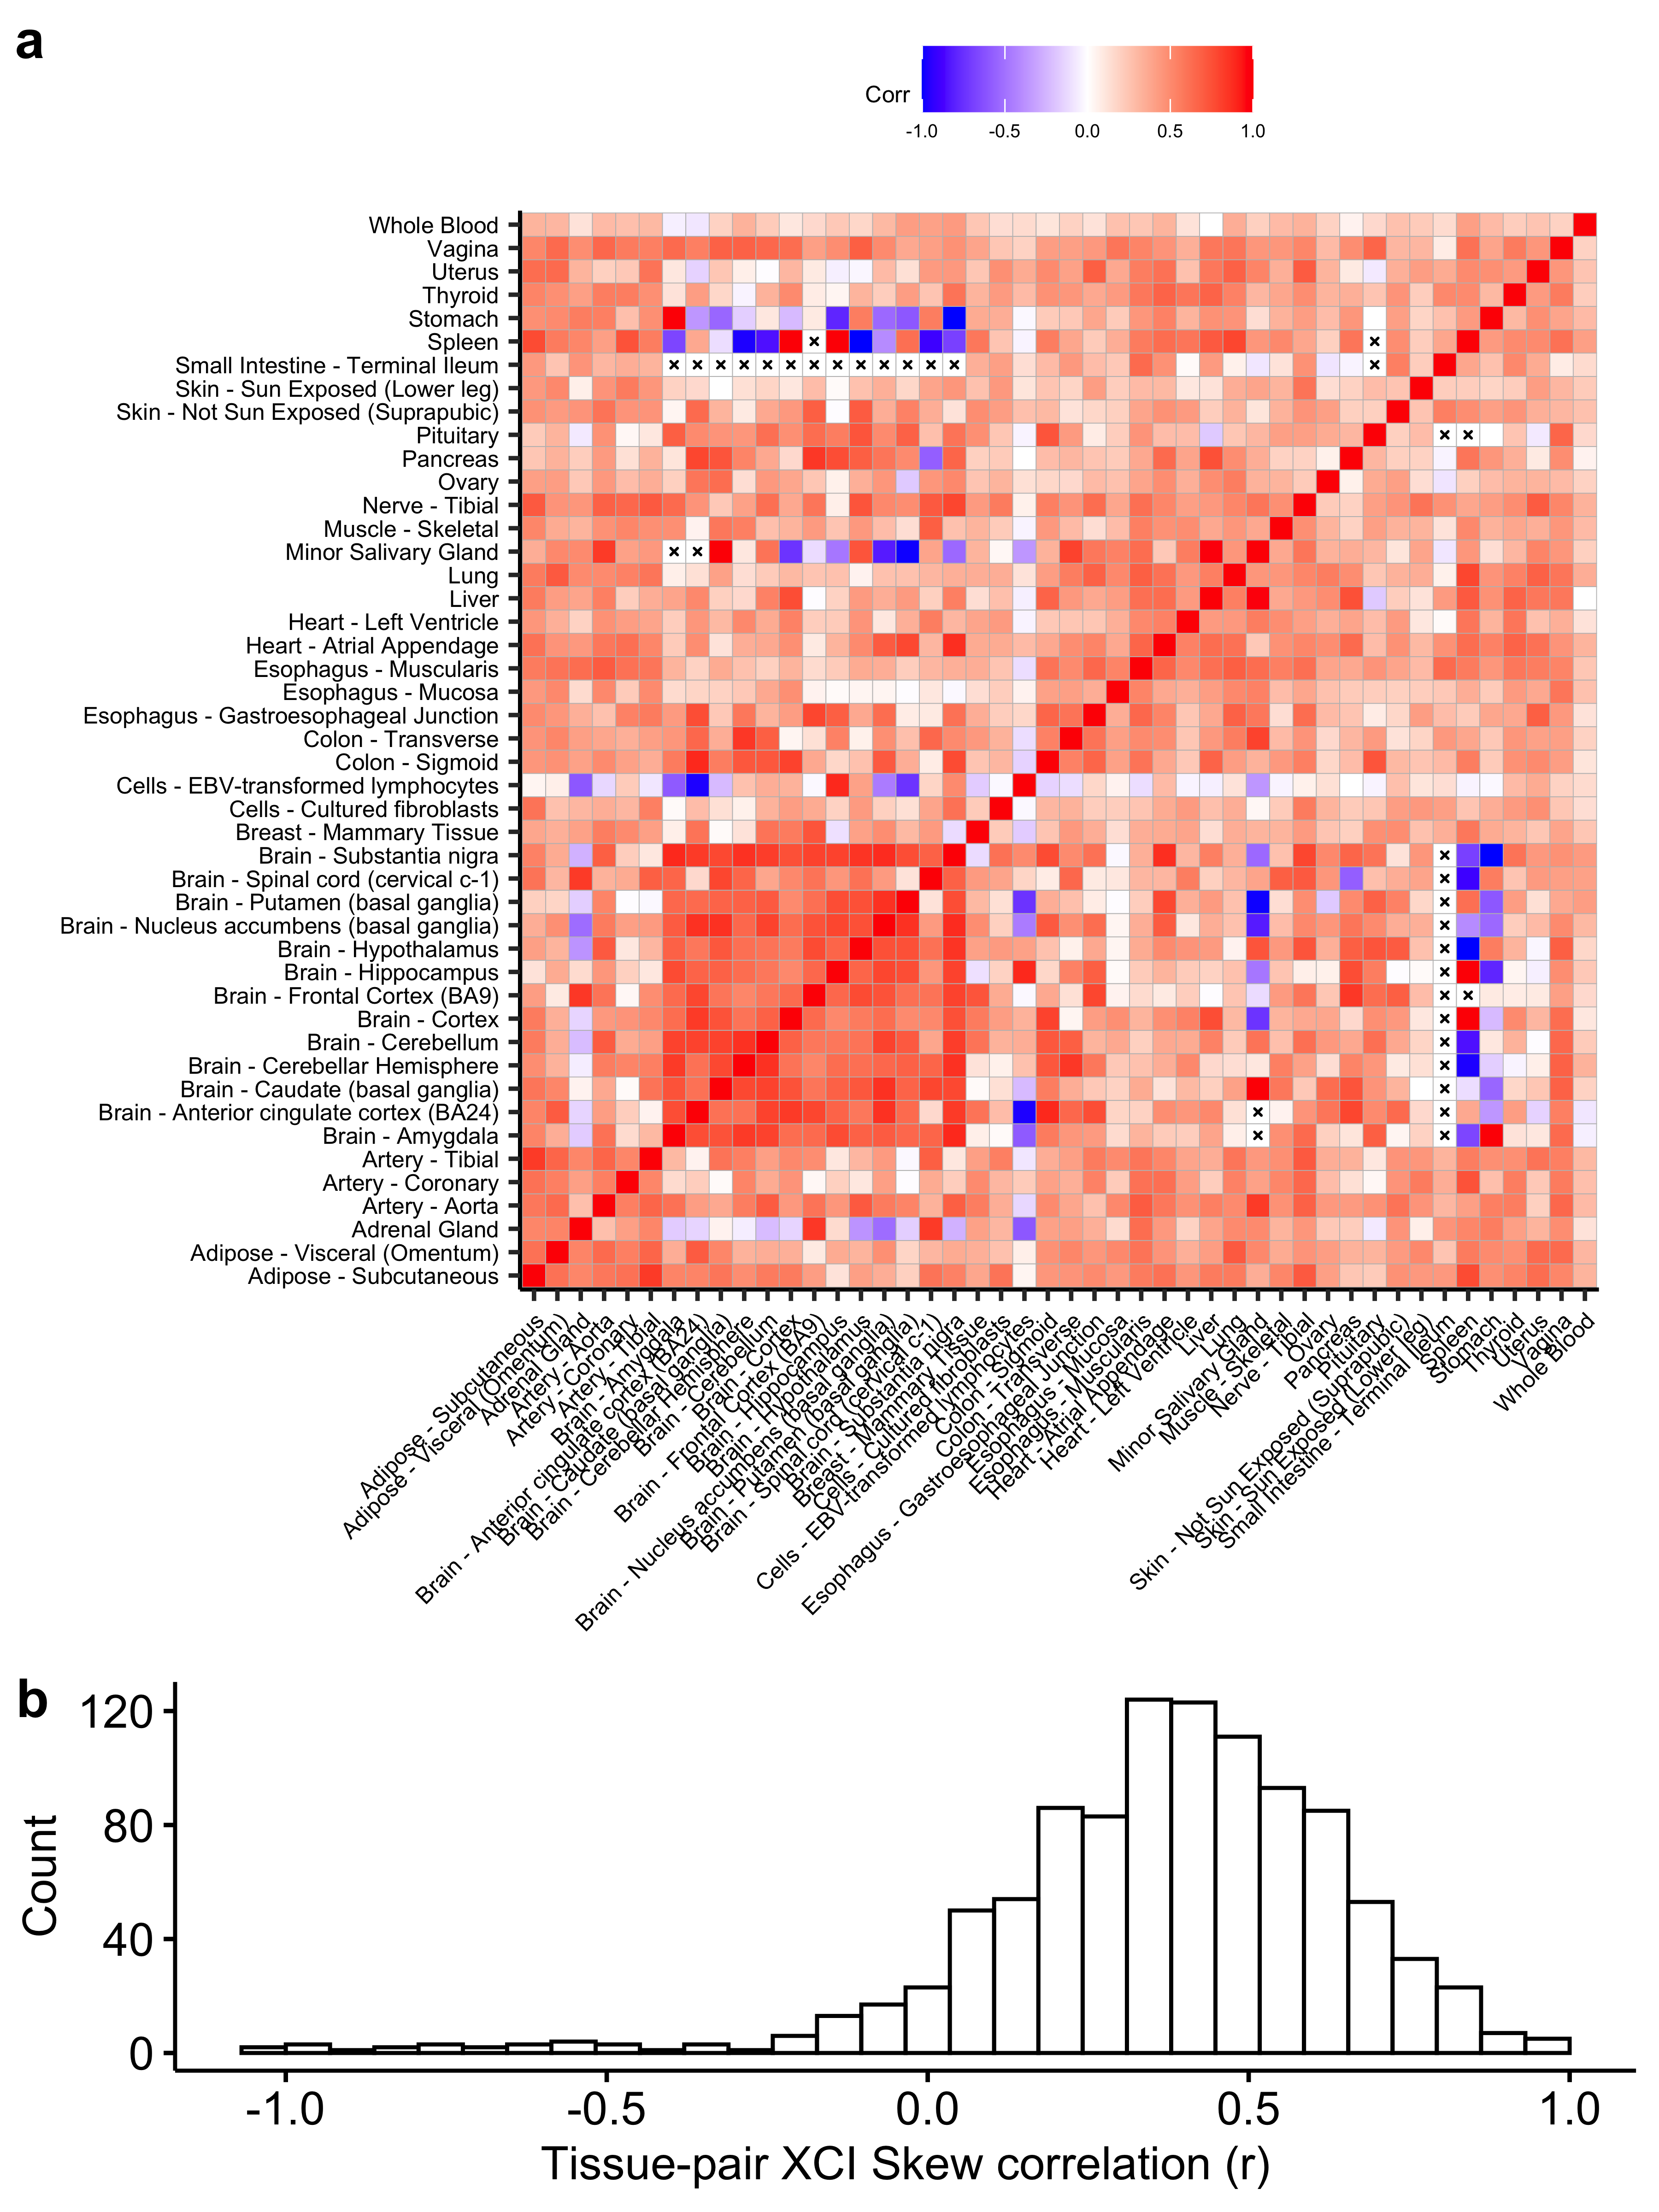
\includegraphics[width=0.75\textwidth]{chapter4/Figures/Supplementary_Figure_2.png}
    \caption{
        Pearson correlation of XCI skew between tissues.
        \textbf{a}, Correlation matrix of tissue-specific XCI skew. White boxes with 'X' symbol indicate that less than 25 observations were available for the tissue pair.
        \textbf{b}, Histogram of correlation between 1,017 non-identical tissue pairs. We observed a mean correlation of 0.3663 and median of 0.3992.
    }
    \label{fig:supp_fig4.2}
\end{figure}

% Inferring XCI skew from expression data can be confounded by both technological and biological factors that may lead to similar associations with our genetic burden scores. Reference bias, the tendency for RNA-seq reads with reference alleles to better map to a reference genome than non-reference alleles \cite{Stevenson2013-cg}, may be a significant confounding variable. This bias is especially relevant to the genetic burden defined by the proportion of alternate alleles carried by a haplotype. For example, an alternate allele may have lower observed expression than the reference allele simply due to reference bias rather than XCI skew. To account for this source of bias, we utilized RNA-seq reads that were aligned with a filter utilizing WASP, a method that accounts for reference bias by mapping reads with swapped genotypes \cite{Van_de_Geijn2015-oy}.
% Regulatory effects of genetic variation may also lead to imbalances in expression measured from each X chromosome that may be erroneously attributed to skew in X chromosome inactivation. To address this source of confounding, we performed similar experiments using the non-acrocentric autosomes (chromosomes with arms of roughly equal size) of the female samples. In short, we calculated skewing at heterozygous sites that were captured by RNA-seq reads on the q or long arm of the autosome. We observed no significant level of average ‘skewing’ in these chromosomes (Figure \ref{fig:supp_fig4.3}). 

% \begin{figure}[ht]
    \centering
    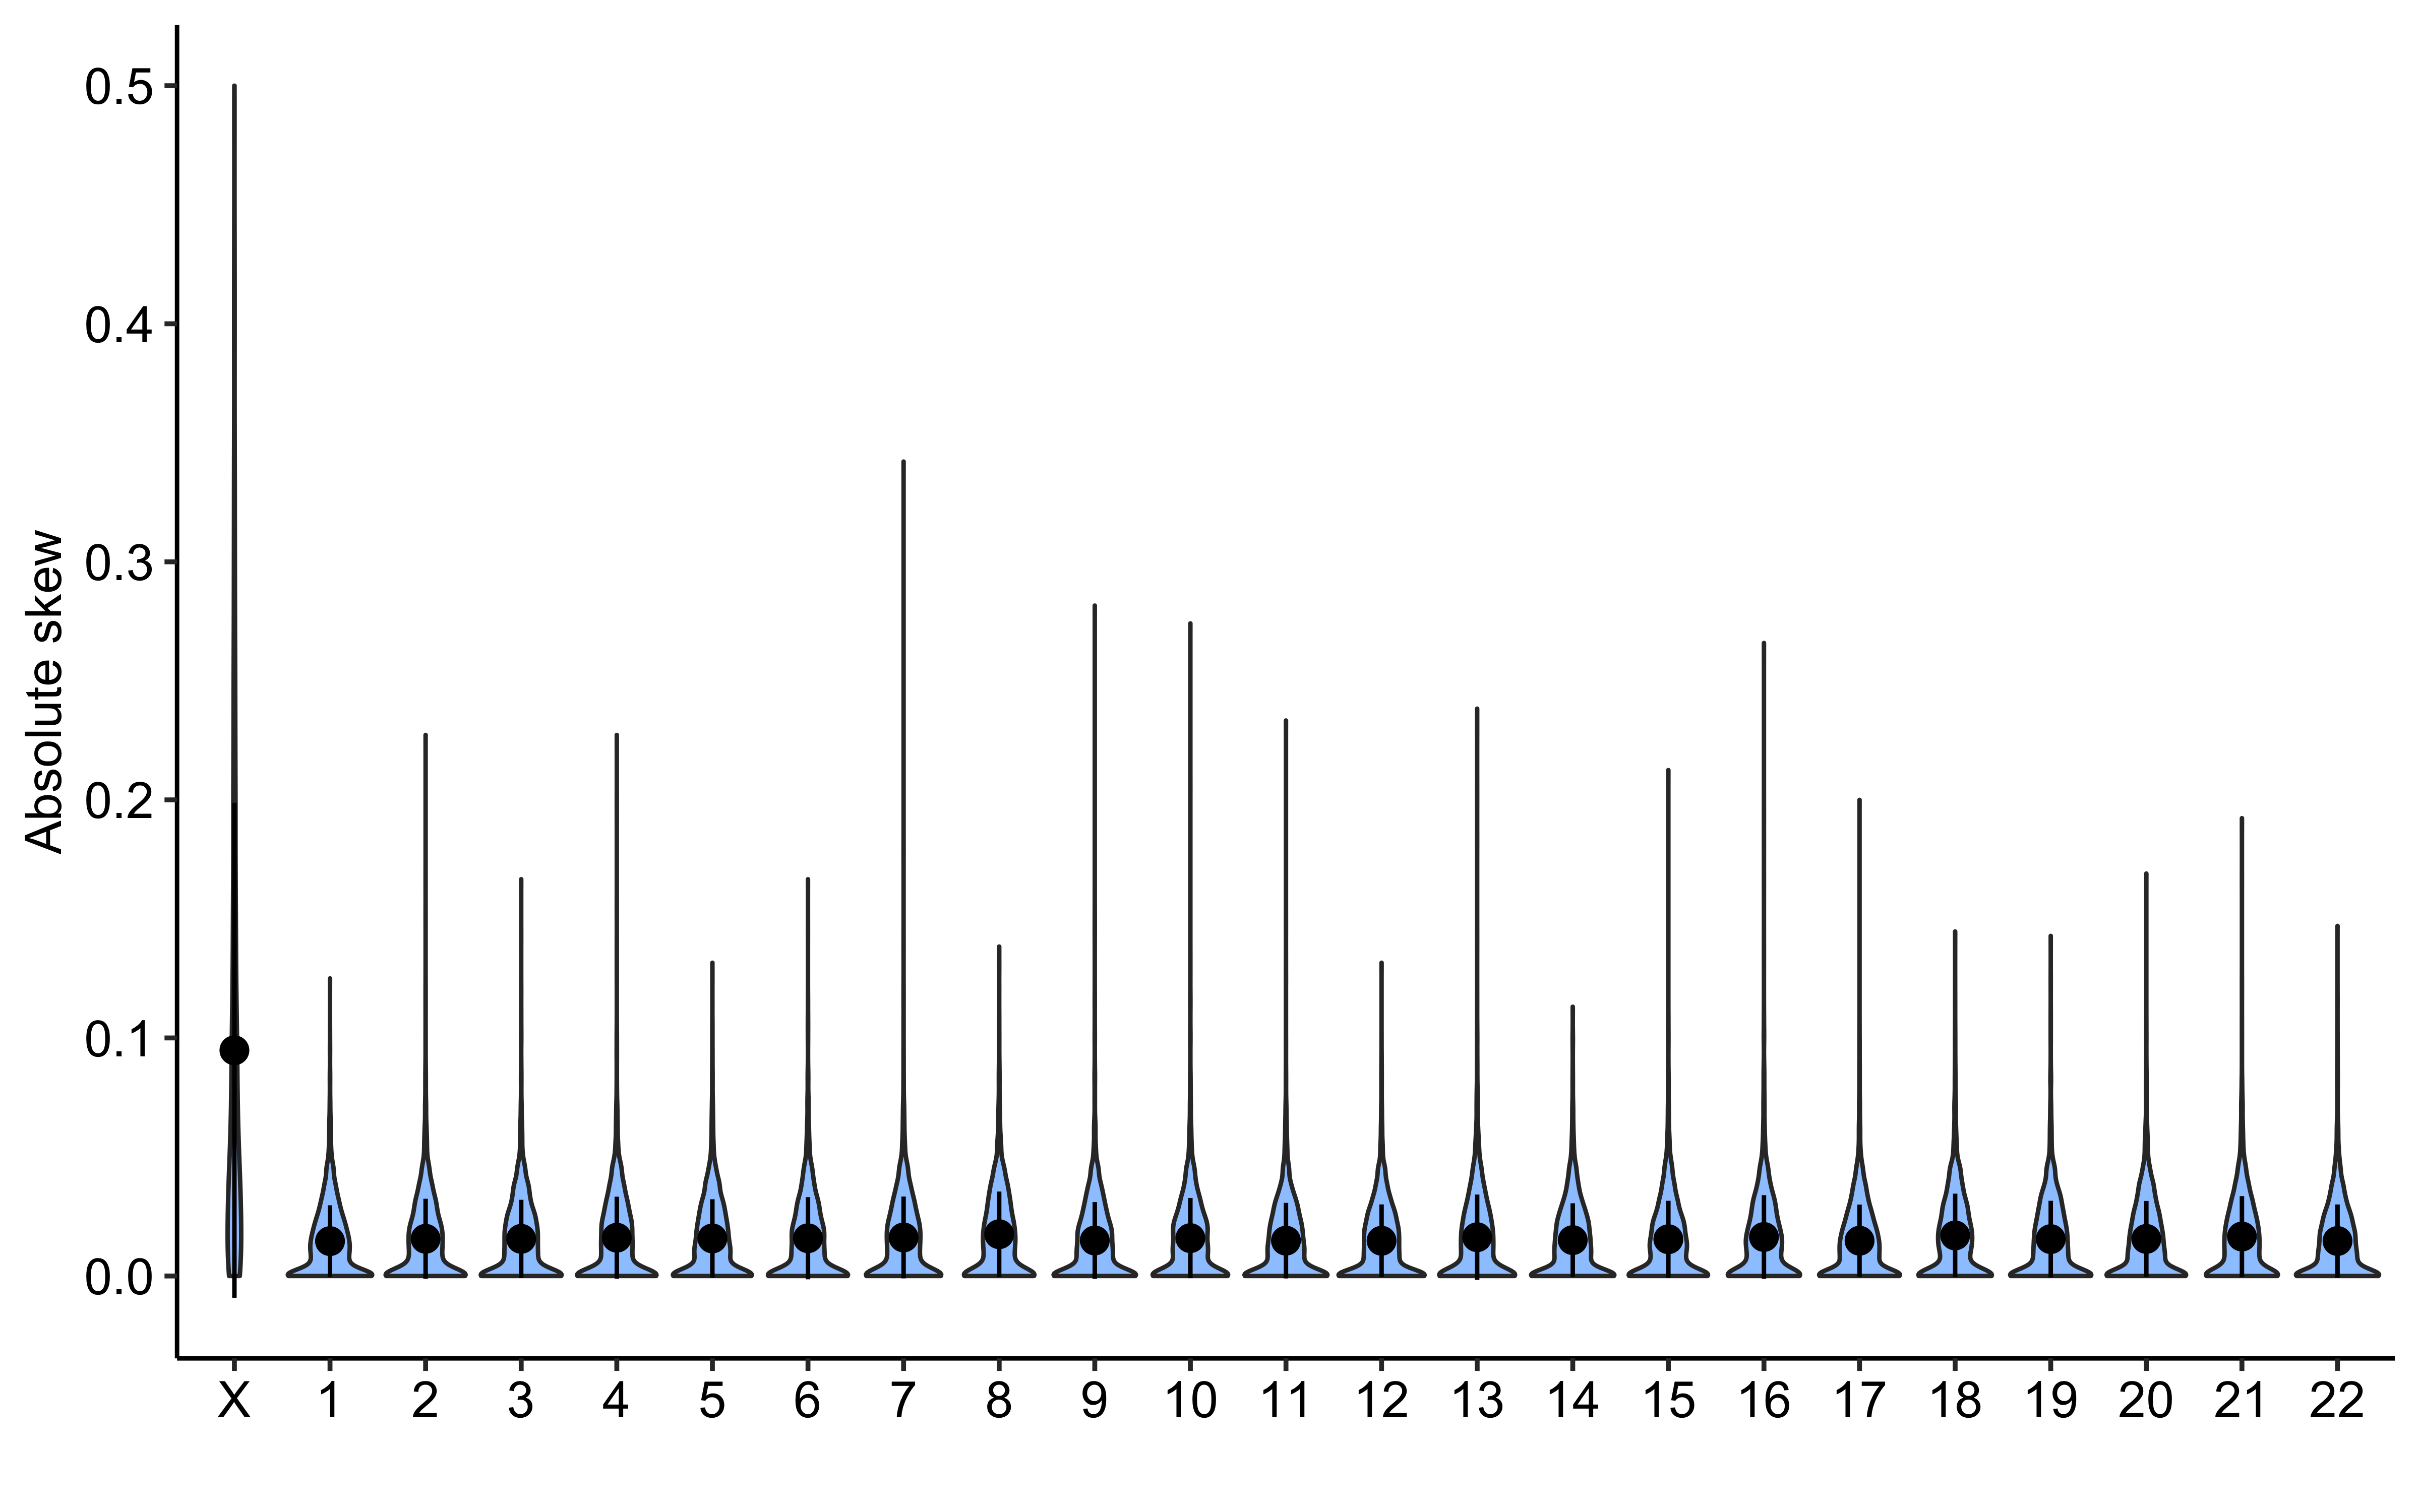
\includegraphics[width=0.75\textwidth]{chapter4/Figures/Supplementary_Figure_3.png}
    \caption{
        Estimated absolute skew in expression at heterozygous sites on the X chromosome and non-acrocentric autosomes. On the X chromosome, this value is used as the estimate of inactivation skewing since heterozygous sites are within fully inactivated genes. On the autosomes, an equal number of heterozygous sites used on the X chromosome for each sample were randomly selected from the q-arm to estimate the median skew in expression. Dots indicate mean of absolute skew with vertical lines indicating one standard deviation.
    }
    \label{fig:supp_fig4.3}
\end{figure}

% We also performed an analysis of the male GTEx samples to test the possibility of regulatory effects rather than skewing in inactivation. Since males only have one X chromosome, we associated genetic features with expression of each gene on the X chromosome. If our genetic scores are associated with downregulation of expression rather than cause XCI skew, we anticipated this experiment to show a significant negative association with the expression of X chromosome genes across males.

% \subsection{Genetic burden is associated with XCI skew}

% We defined the following genetic burden scores for this analysis: the proportion of missense and synonymous mutations carried by each haplotype, and the difference in average CADD score \cite{Rentzsch2019-pk} between the two haplotypes. CADD scores provide a quantitative measure of the predicted deleteriousness of a variant. Only genetic variation outside of the genes that were used to calculate XCI skew were considered in these scores to avoid capturing cis regulatory effects. To associate these burden measures with XCI skew, we fit a linear mixed model with random intercepts accounting for the individual of origin for each tissue sample and tissue type. In this model, the difference in CADD score between haplotypes had a significant negative effect on XCI skew (coefficient = -0.1289 ± 0.0451, p = 0.0023) (Figure \ref{fig:fig4.2}a). This result suggests that a higher genetic burden in terms of deleterious variation is associated with higher rates of inactivation of the haplotype. We found that this association was not significant across the non-acrocentric autosomes (Table \ref{table:table4.1}). In addition, these burden scores were not associated with the regulation of gene expression on the X chromosome in male samples. 

% \begin{figure}[ht]
    \centering
    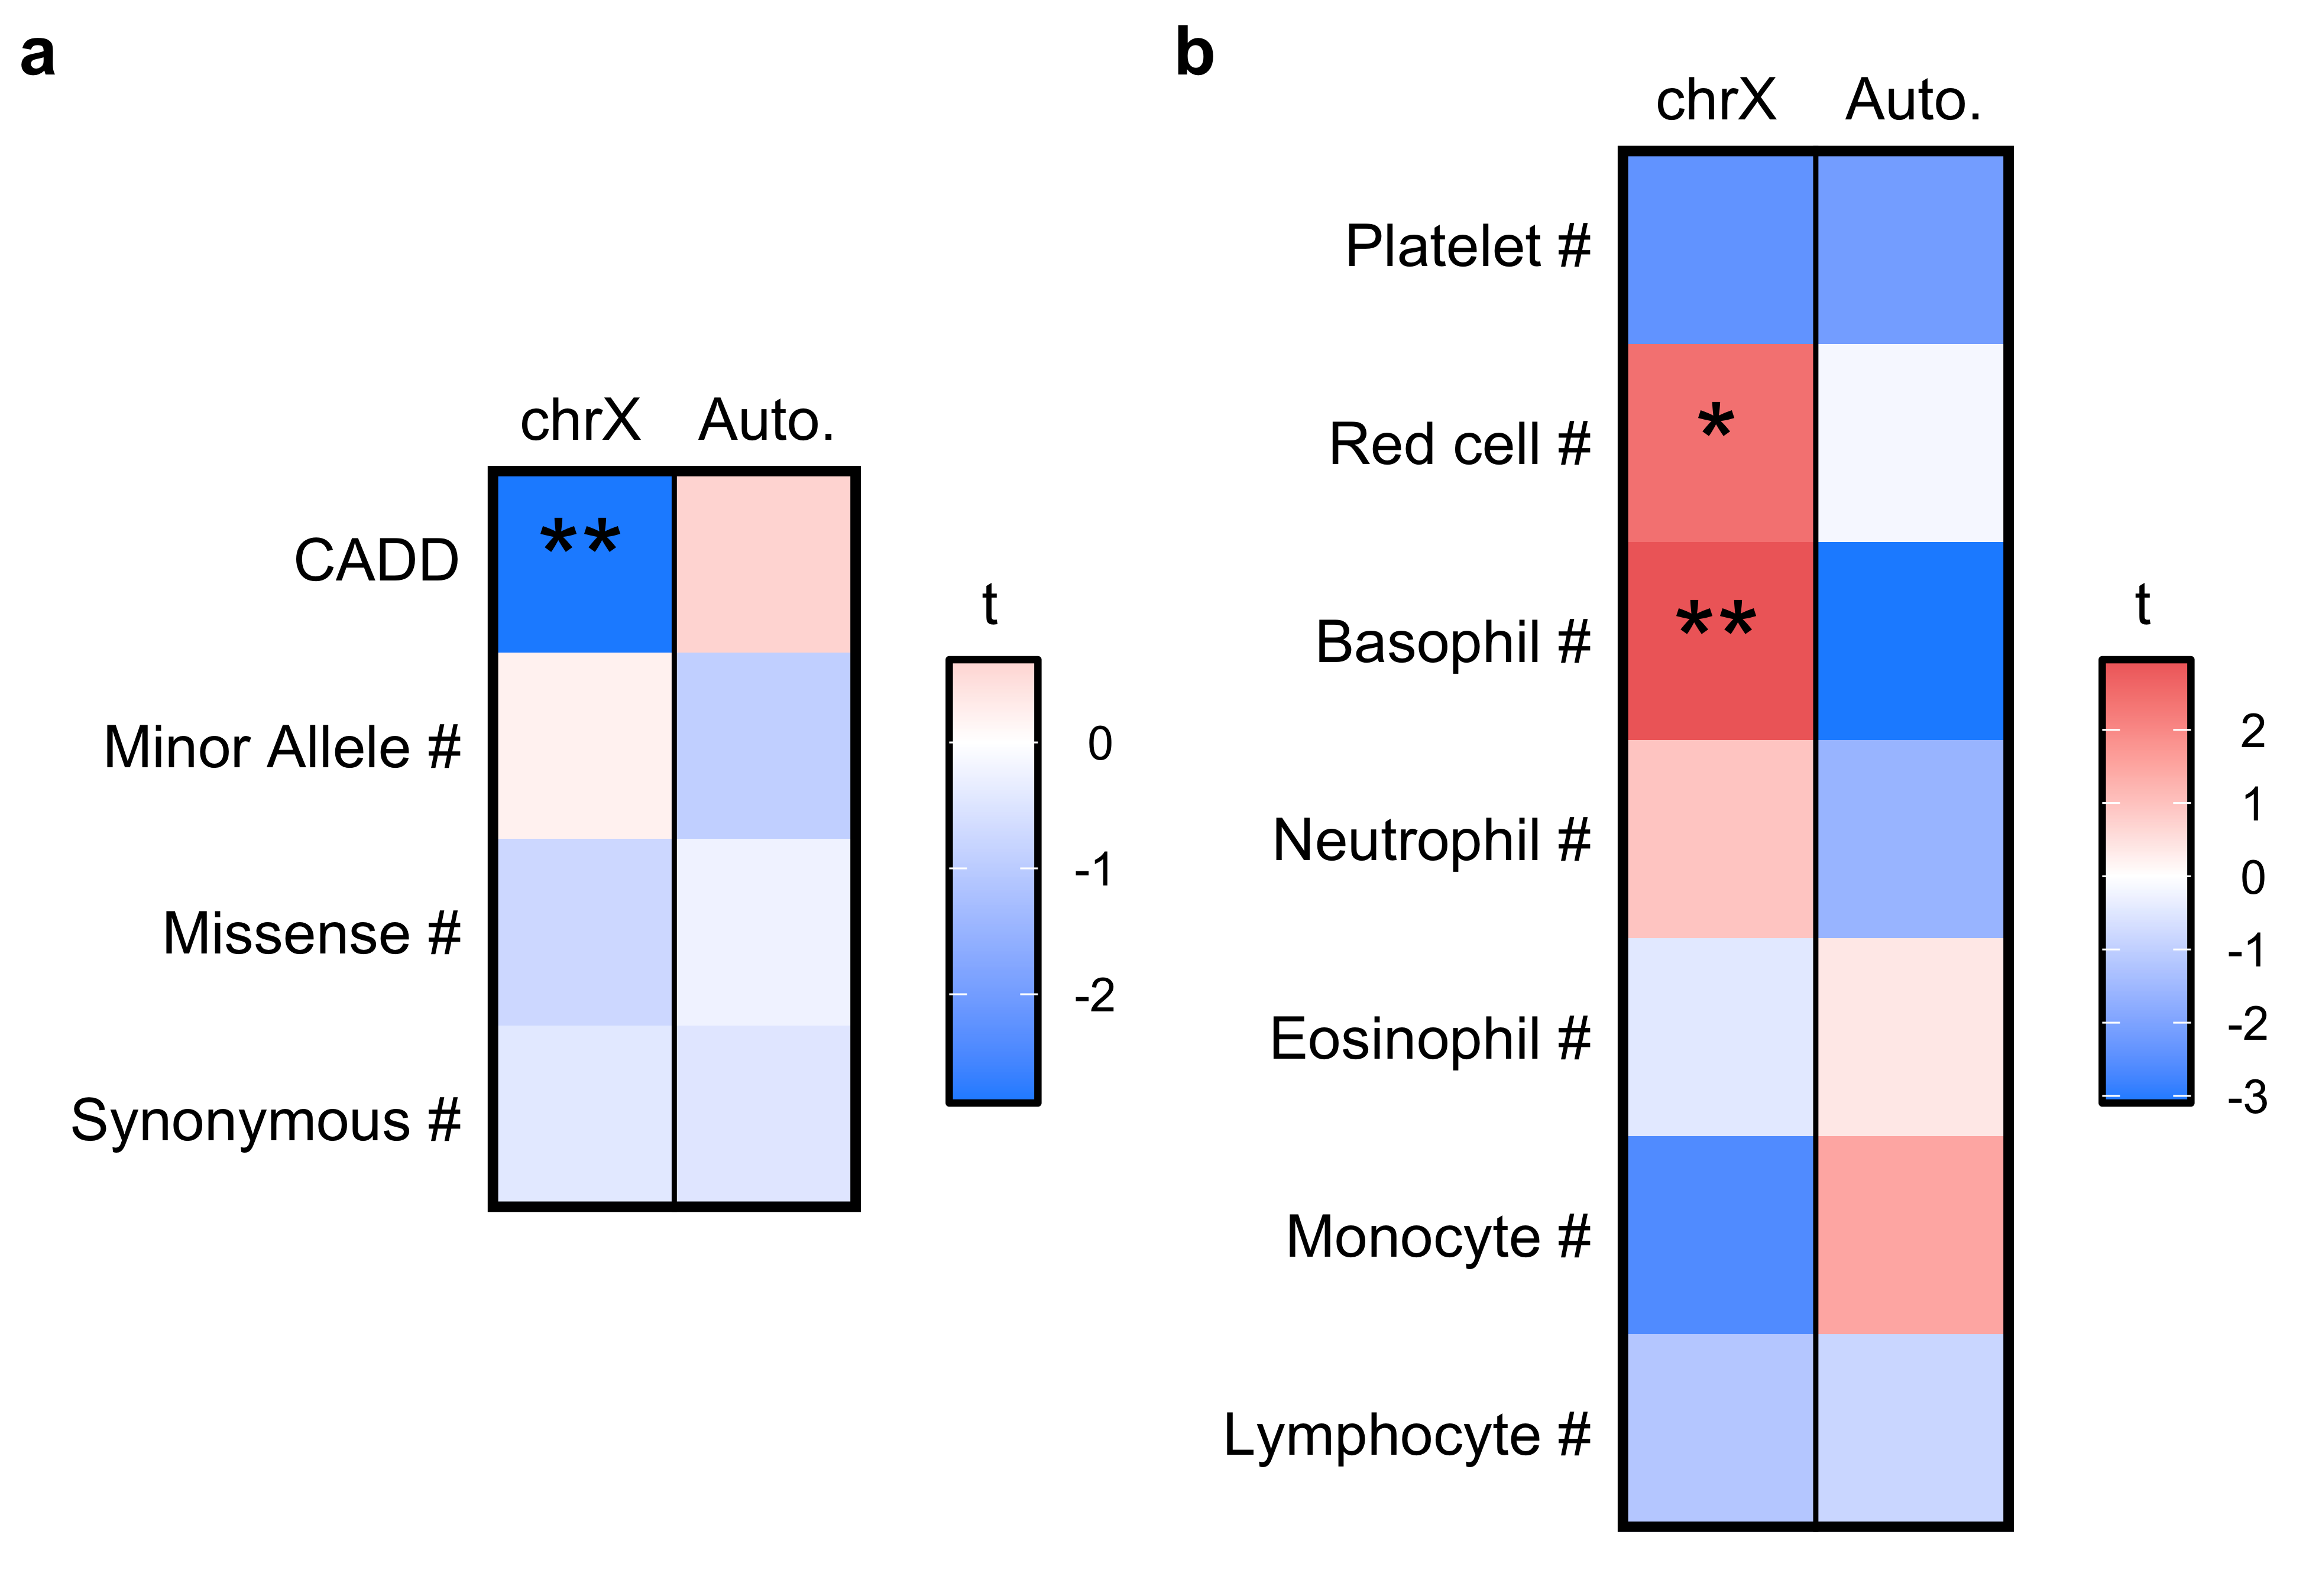
\includegraphics[width=0.5\textwidth]{chapter4/Figures/Figure_2.png}
    \caption{
        Association between genetic scores and skew estimated from expression at heterozygous sites on X chromosome (chrX) and non-acrocentric autosomes (Auto.). Colors indicate the relative t-score from a linear mixed model association test with an asterisks (*) indicating significance at $\alpha=0.05$ and double asterisks (**) indicating significance after Bonferroni correction.
        \textbf{a}, Association results of genetic burden scores with estimated skew. A one-sided t-test was performed under the assumption that increased genetic burden decreases skew towards the haplotype. CADD indicates difference in mean CADD score of each haplotype. The remaining scores compare the number of the indicated mutations on each haplotype.
        \textbf{b}, Association results of proliferative polygenic scores with estimated skew. Counts of different blood cell types were used as a proxy for proliferative potential. A one-sided t-test was performed under the assumption that increased proliferation genetic scores will increase skew towards the haplotype.}
    \label{fig:fig4.2}
\end{figure}
% \begin{table}[ht]
\scriptsize
\caption{Burden associations with skewing in XCI and autosomal q-arm expression}
\centering
\begin{tabular}{llllll}
  \hline
 Burden Score & Chromosome(s) & $\beta$ (s.e.) & df & $t$ & $P$ \\ 
  \hline
CADD & chrX & -0.1289 (0.0451) & 240.6684 & -2.8579 & 0.0023 \\ 
   & Auto. & 0.0024 (0.0037) & 60762.2663 & 0.6516 & 0.7427 \\ 
  Minor Allele \# & chrX & 0.0097 (0.0453) & 240.5593 & 0.2141 & 0.5847 \\ 
   & Auto. & -0.0034 (0.0037) & 58076.8103 & -0.9263 & 0.1772 \\ 
  Missense \# & chrX & -0.0355 (0.0476) & 238.7277 & -0.7452 & 0.2285 \\ 
   & Auto. & -0.0009 (0.0037) & 59330.7798 & -0.2314 & 0.4085 \\ 
  Synonymous \# & chrX & -0.0202 (0.0463) & 239.3741 & -0.4356 & 0.3318 \\ 
   & Auto. & -0.0018 (0.0037) & 39637.5931 & -0.4748 & 0.3175 \\ 
   \hline
\end{tabular}
\label{table:table4.1}
\end{table}

% \subsection{Variation in proliferation-related polygenic scores is associated with XCI Skew}

% We utilized publicly available polygenic risk score weights to calculate the proliferative potential of each haplotype in the female samples. Specifically, we used various blood cell counts as phenotypes under the assumption that these scores are concordant with hematopoiesis and proliferative cell activity \cite{Loh2020-mb}. We found that the haplotype with the higher red blood cell polygenic score (coefficient = 0.1116 ± 0.0462, p = 0.0082) and basophil polygenic score (coefficient = 0.1355 ± 0.0460, p = 0.0018) tends to be overrepresented in terms of XCI skewing (Figure \ref{fig:fig4.2}b). These results imply that higher proliferative-related polygenic scores are associated with an enrichment for cells with this haplotype active across tissues. We also ran similar autosomal and male analyses to test the alternative hypothesis that these polygenic scores may be capturing gene regulatory effects. We found no significant associations between these scores in the female non-acrocentric autosomes (Supplementary Table \ref{table:table4.2}). In the analysis of male samples, the basophil polygenic score was significantly associated with increased expression of AFF2 in 4 tissues (Supplementary Table \ref{table:table4.4}). However, this gene is considered a variable XCI escape gene and therefore was not used to calculate XCI skew in the female samples.

% \begin{table}[ht]
\scriptsize
\caption{Proliferation-related polygenic score associations with skewing in XCI and autosomal q-arm expression}
\centering
\begin{tabular}{llllll}
  \hline
Polygenic Score & Chromosome(s) & $\beta$ (s.e.) & df & $t$ & $P$ \\ 
  \hline
Platelet \# & chrX & -0.1093 (0.0456) & 240.8663 & -2.3997 & 0.9914 \\ 
   & Auto. & -0.0079 (0.0037) & 58466.4918 & -2.1498 & 0.9842 \\ 
  Red cell \# & chrX & 0.1116 (0.0462) & 238.7682 & 2.4172 & 0.0082 \\ 
   & Auto. & -0.0006 (0.0037) & 54155.3786 & -0.1623 & 0.5645 \\ 
  Basophil \# & chrX & 0.1355 (0.0460) & 237.3432 & 2.9487 & 0.0018 \\ 
   & Auto. & -0.0113 (0.0037) & 60017.3402 & -3.0875 & 0.9990 \\ 
  Neutrophil \# & chrX & 0.0451 (0.0469) & 238.1159 & 0.9606 & 0.1689 \\ 
   & Auto. & -0.0059 (0.0037) & 57022.3082 & -1.6151 & 0.9469 \\ 
  Eosinophil \# & chrX & -0.0224 (0.0475) & 238.1788 & -0.4710 & 0.6810 \\ 
   & Auto. & 0.0014 (0.0037) & 60407.8660 & 0.3883 & 0.3489 \\ 
  Monocyte \# & chrX & -0.1209 (0.0463) & 237.1836 & -2.6126 & 0.9952 \\ 
   & Auto. & 0.0055 (0.0037) & 50177.1222 & 1.4848 & 0.0688 \\ 
  Lymphocyte \# & chrX & -0.0560 (0.0473) & 238.1101 & -1.1834 & 0.8811 \\ 
   & Auto. & -0.0031 (0.0037) & 57465.9629 & -0.8419 & 0.8001 \\ 
   \hline
\end{tabular}
\label{table:table4.2}
\end{table}


% \begin{table}[ht]
\scriptsize
\caption{Covariates associated with chromosome X gene regulation in males.}
\centering
\begin{tabular}{lllllllll}
  \hline
 Covariate & Gene Name & Gene ID & XCI status & Tissue & $\beta$ (s.e.) & $P$ & $Q$ \\ %& $N$ \\ 
  \hline
  Basophil \# & AFF2 & ENSG00000155966.13 & Variable & Adipose (Subc.) & 0.1522 (0.0329) & 5.701e-06 & 0.0490 \\ % & 329 \\ 
  &  &  &  & Lung & 0.1825 (0.0374) & 1.841e-06 & 0.0317 \\ %& 302 \\ 
  &  & &  & Skin (Sup.) & 0.1616 (0.0344) & 4.353e-06 & 0.0490 \\ %& 297 \\ 
   &  &  &  & Thyroid & 0.1499 (0.0296) & 7.902e-07 & 0.0272 \\ %& 324 \\ 
  rs141680486 & TMEM187 & ENSG00000177854.7 & Inactive &  EBV lymphocytes & -0.3917 (0.0696) & 8.734e-07 & 0.0302 \\ %&  73 \\ 
   \hline
\end{tabular}
\label{table:table4.4}
\end{table}

% \subsection{Variation in specific loci is significantly associated with XCI skew}

% While the previous analyses suggest that genetic burden and proliferative potential is associated with skewed XCI, they do not provide specific variants or loci that contribute to this association. We performed an association study on the X chromosome to address this question. Specifically, we associated variants on the X chromosome with the absolute XCI skew measurements (Figure \ref{fig:fig4.3}a). We found 2 variants that were significant at a FDR of 0.05 (Table \ref{table:table4.3}). The first variant (rs141680486) is an intronic SNP found within the DMD gene, also known as dystrophin, and was significantly associated with increased absolute XCI skew (coefficient = 0.0203 ± 0.0041, p=7.978e-07). We observed large absolute skew in samples that were heterozygous for this variant compared to those who were homozygous (Figure \ref{fig:fig4.3}b). Moreover, we found that the haplotype with the minor allele tends to be more inactivated than the other haplotype in heterozygous samples (Figure \ref{fig:fig4.3}c). The second variant (rs73227260) is an intronic SNP in LOC101928359, a non-coding transcript,  and was also associated with increased absolute XCI skew (coefficient = 0.0199 ± 0.0041, p = 1.265e-06). We observed a high level of skewing in heterozygous individuals with no clear difference in directional skewing depending on the haplotype carrying the minor allele (Figure \ref{fig:supp_fig4.4}).

% Since eQTLs may also cause skewing in expression within cells, we tested the association between these variants and gene expression on the X chromosome in males. We found that the DMD variant (rs141680486) is a significant eQTL for TMEM187 expression in EBV-transformed lymphocytes (coefficient = -0.3917 ± 0.0696, p=8.734e-07). However, we note that these lymphocyte samples were excluded from our female analyses due to extreme XCI skewing. 

% \begin{figure}[ht!]
    \centering
    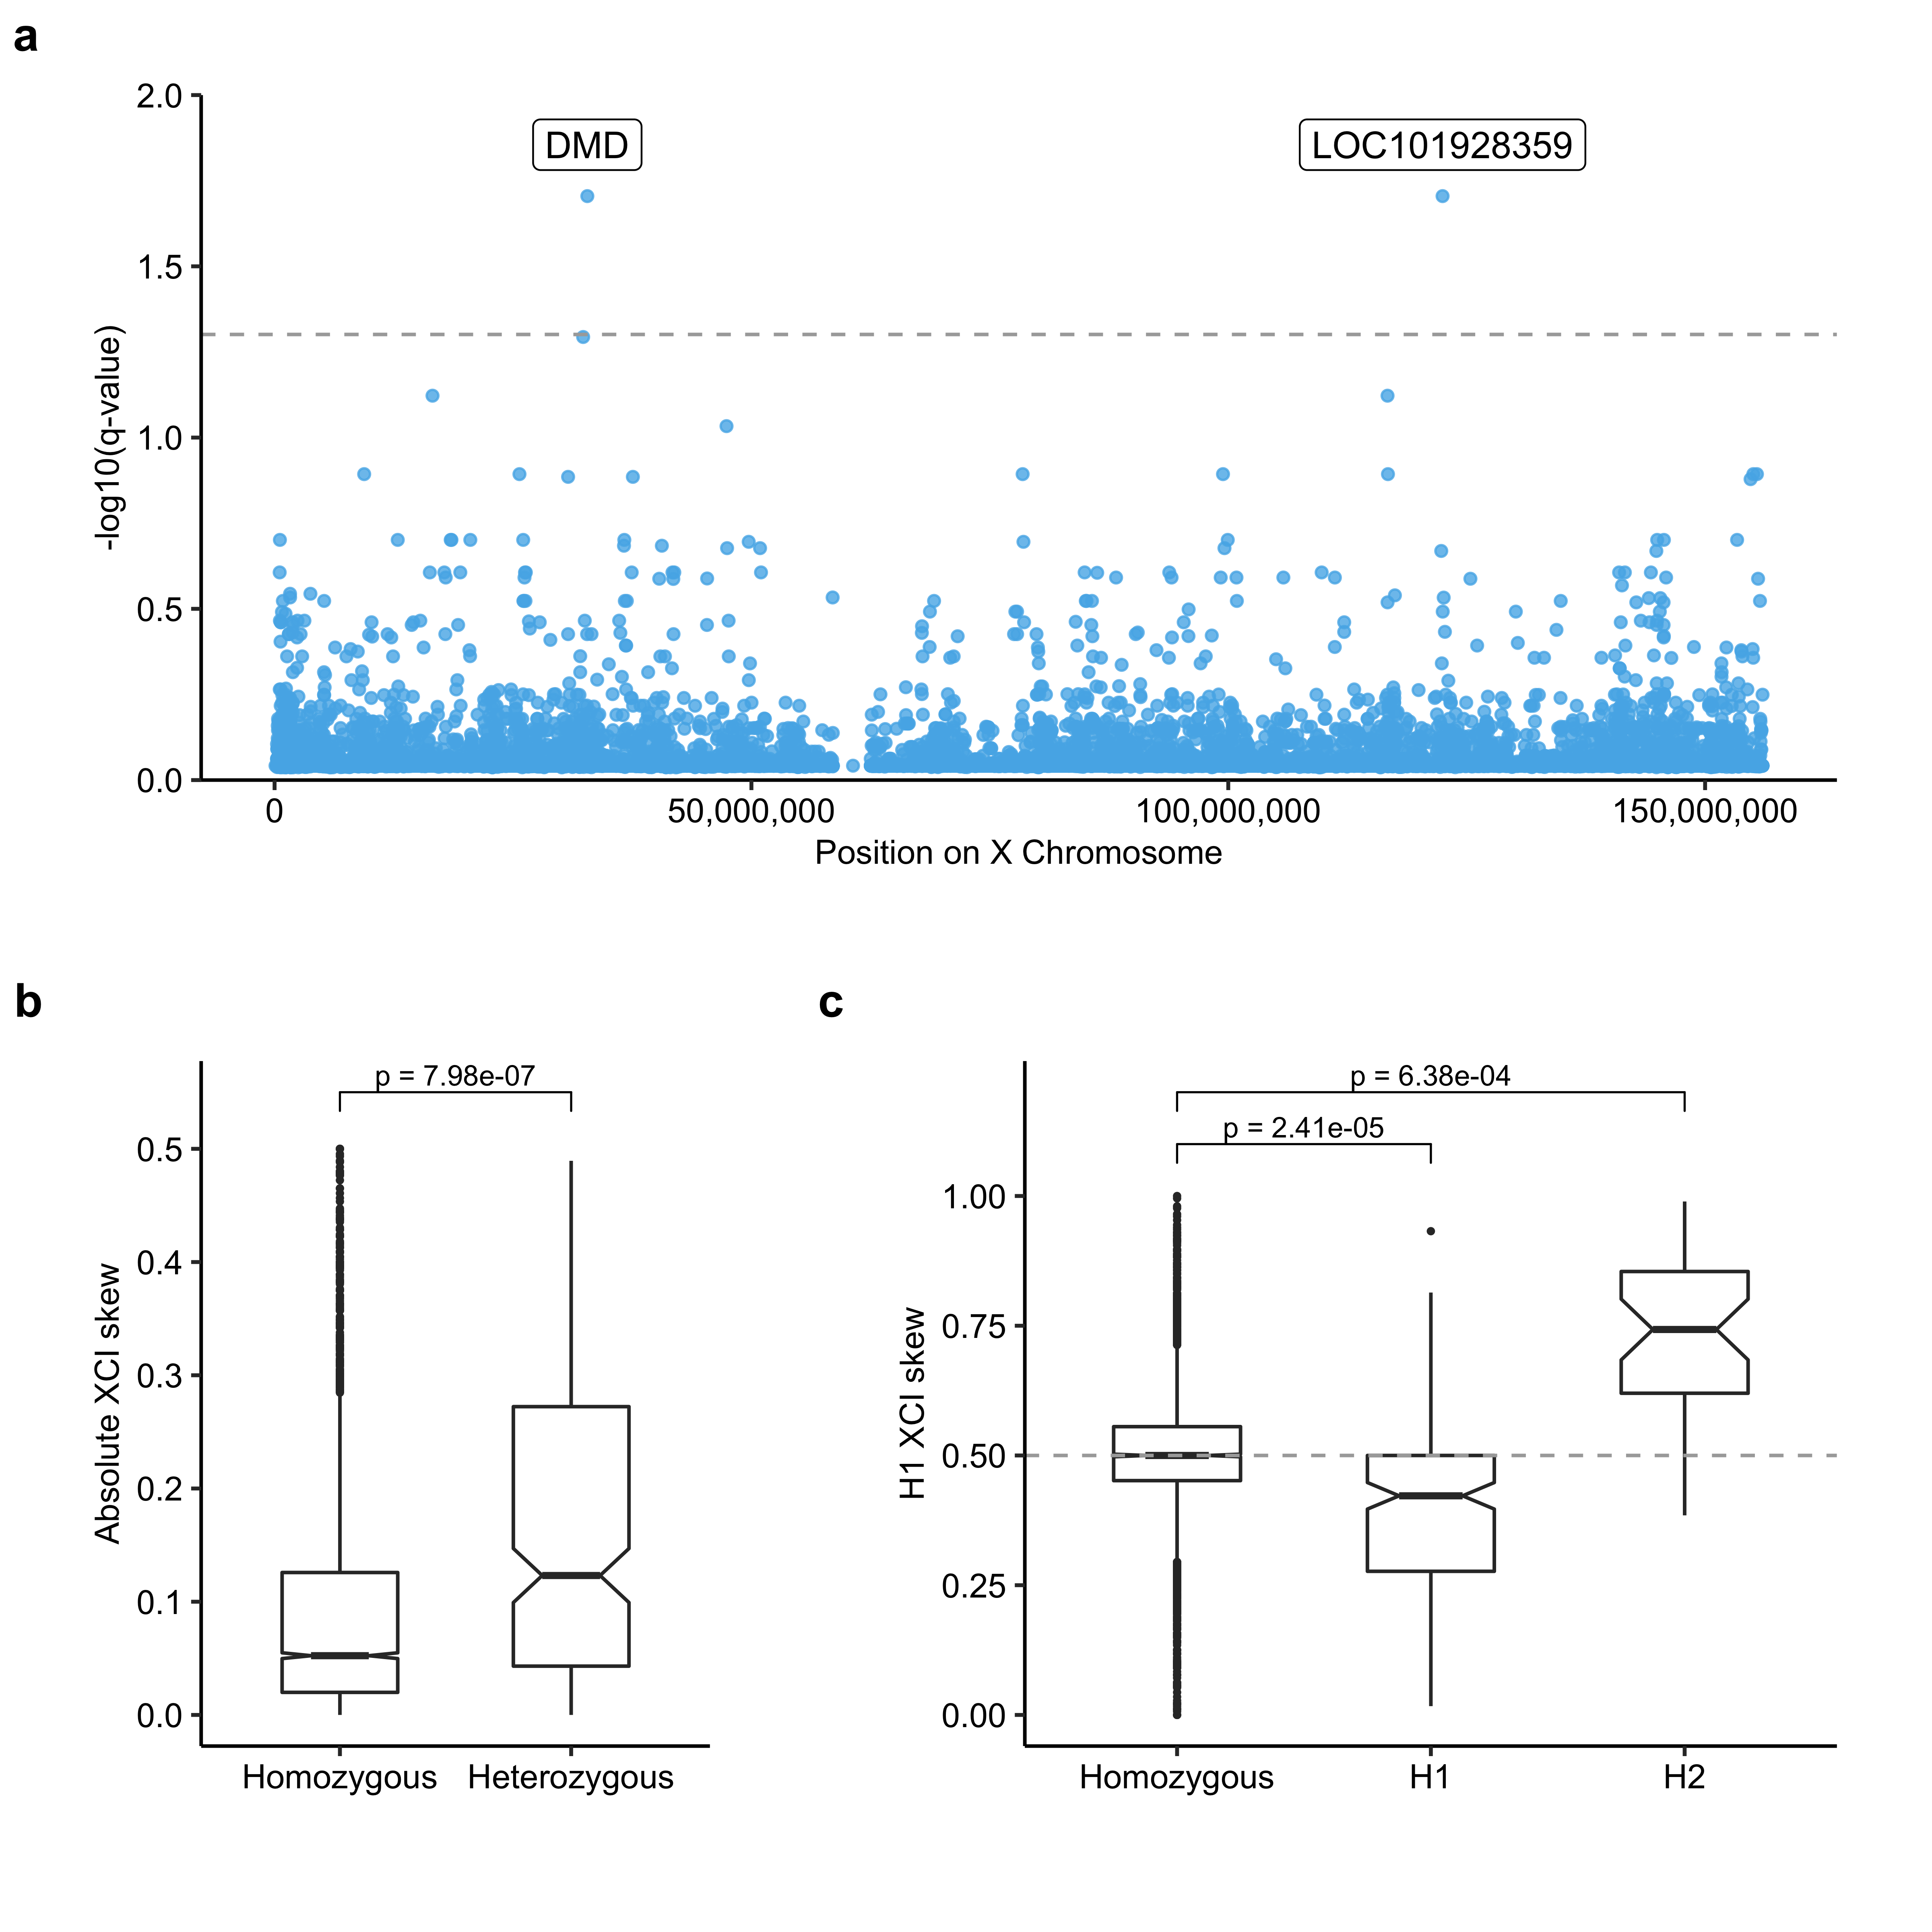
\includegraphics[width=0.75\textwidth]{chapter4/Figures/Figure_3.png}
    \caption{
        Associating specific variation on the X chromosome with inactivation skew. 
        \textbf{a}, Manhattan plot of -log10(q-values) generated from a linear mixed model associating absolute XCI skew with heterozygous status, accounting for age as well as individual and tissue groupings of samples. A one-sided test was performed under the hypothesis that heterozygous status increases absolute skew. Dotted horizontal line indicates local false discovery rate of 0.05. 
        \textbf{b}, Boxplot of absolute XCI skew in samples that are homozygous  (n = 4,232) or heterozygous (n = 230) for the DMD variant (rs141680486). Indicated p-value is from the model described above.
        \textbf{c}, Boxplot of skewing toward haplotype 1 (H1), where the grouping on the x-axis describes individuals without the DMD variant (Homozygous, n = 4,232), with the variant on haplotype 1 (H1, n = 190), and with the variant on haplotype 2 (H2, n = 40). Indicated p-values are from the model described above but with a two-sided test, since we do not assume the direction of skewing associated with a specific variant.}
    \label{fig:fig4.3}
\end{figure}
% \begin{figure}[ht!]
    \centering
    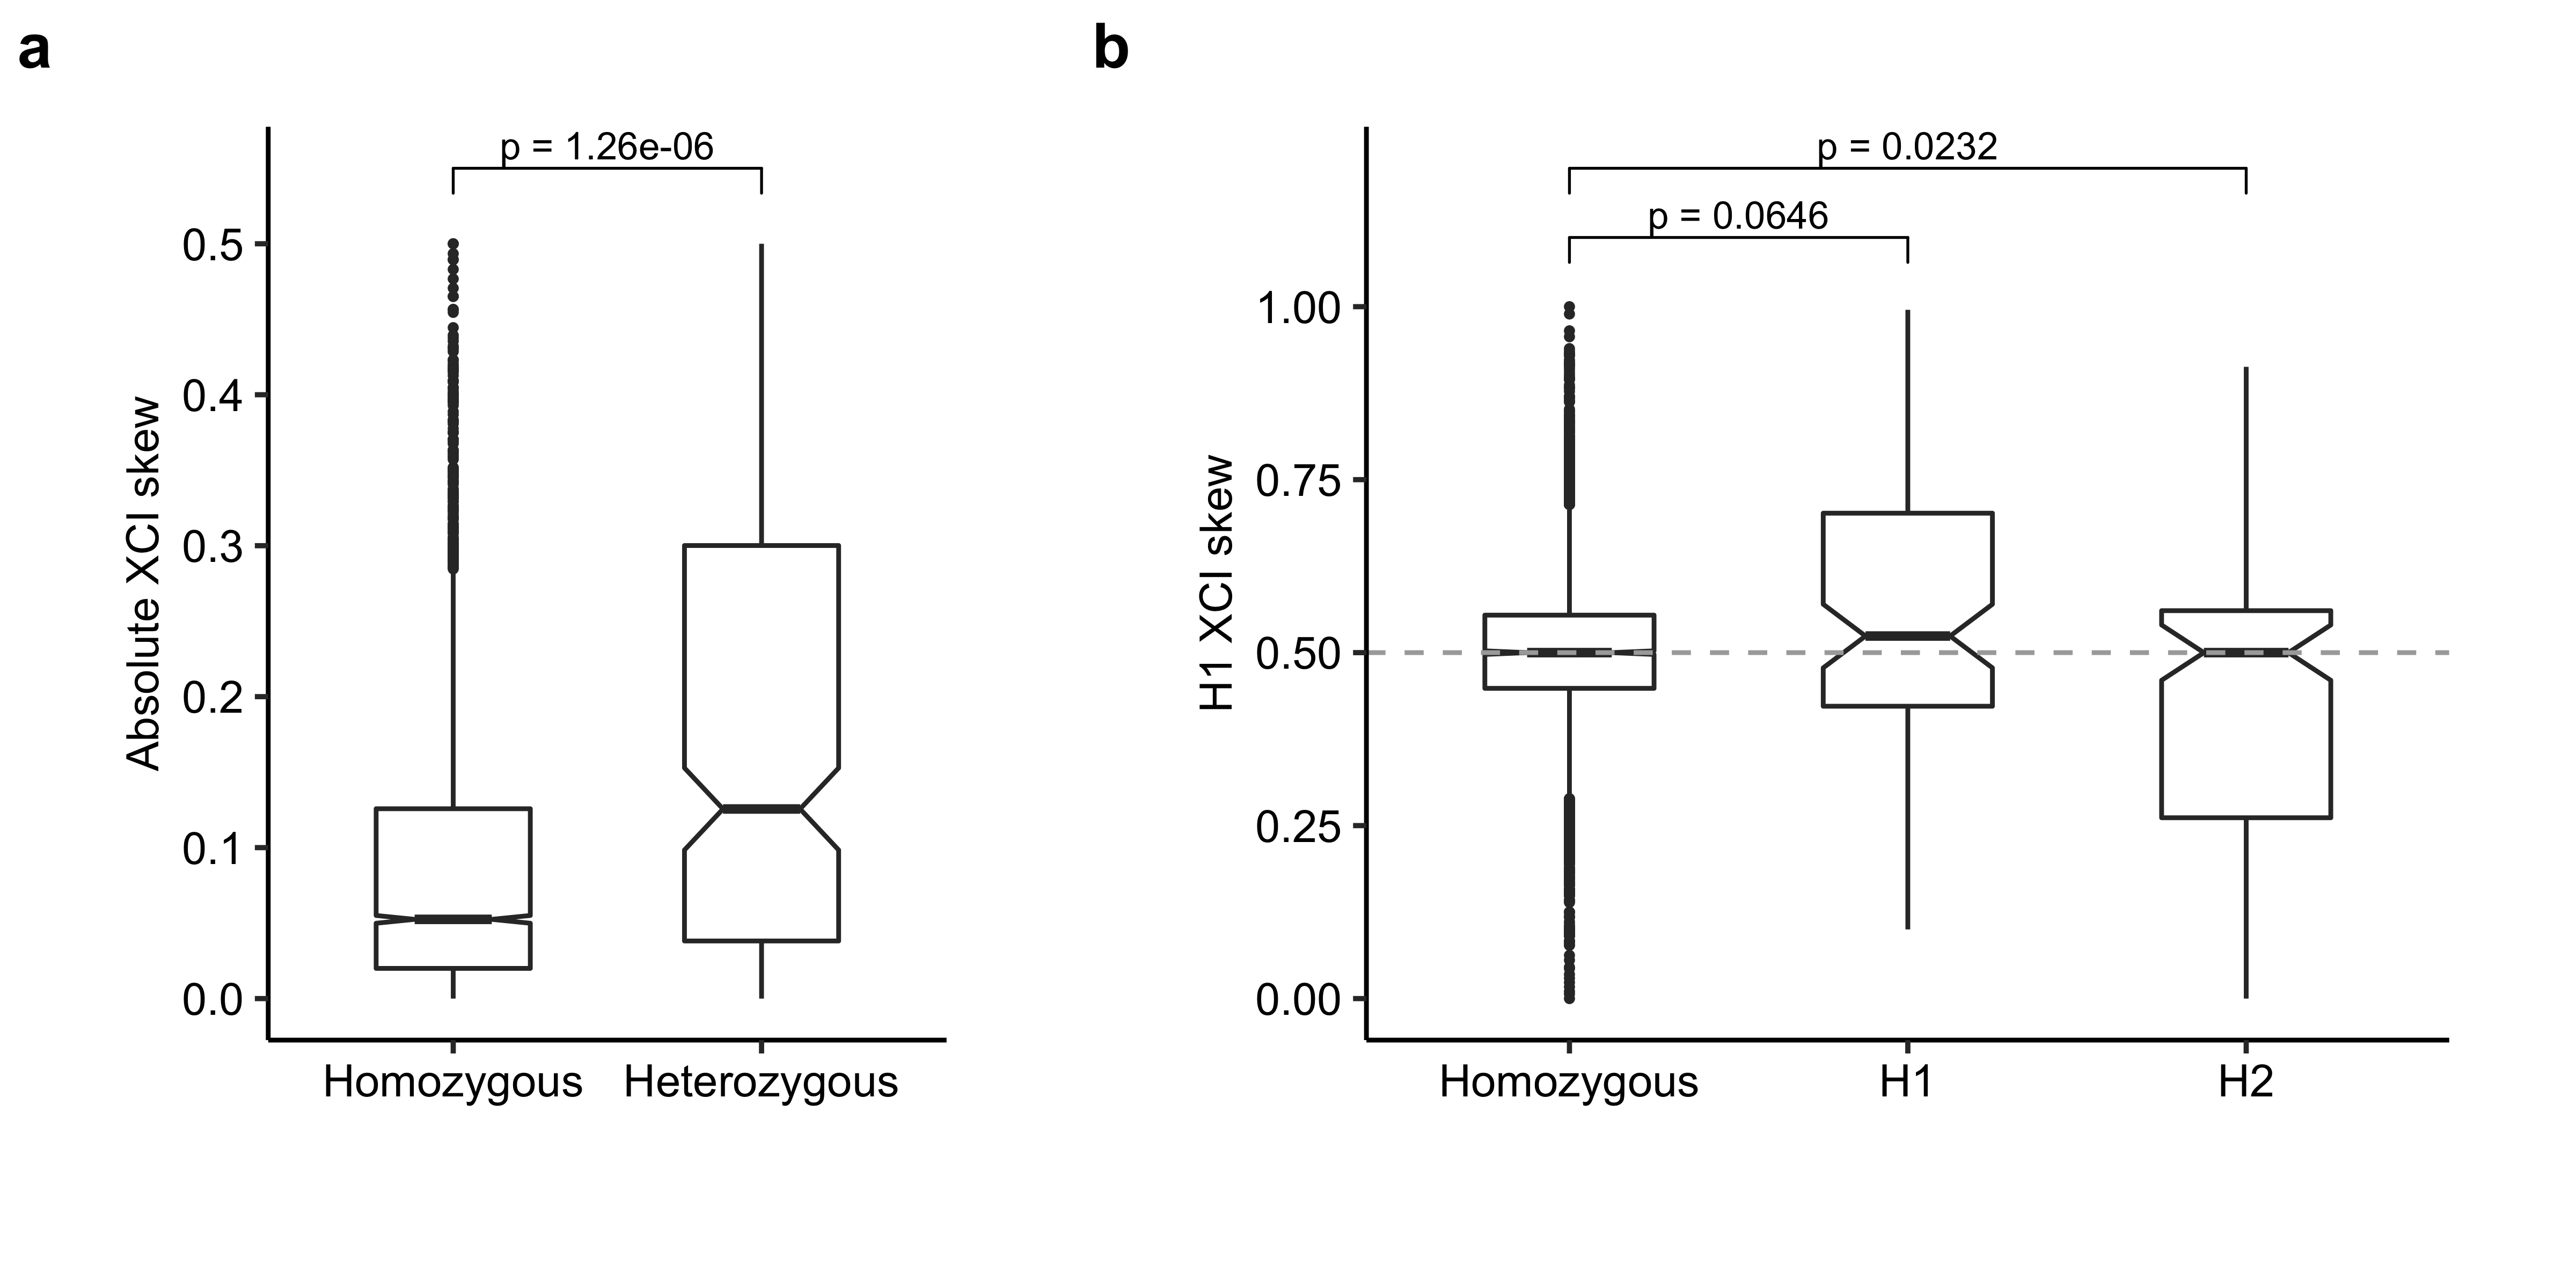
\includegraphics[width=0.9\textwidth]{chapter4/Figures/Supplementary_Figure_4.png}
    \caption{
        Association of LOC101928359 variant (rs73227260) variants with XCI skew. Indicated p-values are from a linear mixed model accounting for individual and tissue of origin.
        \textbf{a}, Boxplot of absolute XCI skew in homozygous samples (n = 4,230) and heterozygous samples (n = 232). Indicated p-value is from a one-sided t-test.
        \textbf{b}, Boxplot of skewing toward haplotype 1 (H1), where the grouping on the x-axis describes individuals without the LOC variant (Homozygous, n = 4,230), with the variant on haplotype 1 (H1, n = 92), and with the variant on haplotype 2 (H2, n = 140). Indicated p-values are from two-sided t-test.  
    }
    \label{fig:supp_fig4.4}
\end{figure}
% \begin{table}[ht]
\scriptsize
\caption{Top 10 variants associated with absolute skewing in XCI}
\centering
\begin{tabular}{lllllll}
  \hline
Locus & SNP & Position & Alleles & AF & $\beta$ (s.e.) & $P_{\text{one-sided}}$ \\ 
  \hline
  DMD & rs141680486 & 32794582 & C/G & 0.0179 & 0.0203 (0.0041) & 7.978e-07 \\ 
  LOC101928359 & rs73227260 & 122471389 & C/T & 0.0203 & 0.0199 (0.0041) & 1.265e-06 \\ 
  DMD & rs144615018 & 32355895 & C/G & 0.0328 & 0.0175 (0.0039) & 4.891e-06 \\ 
  None & rs140456300 & 116700067 & A/T & 0.0316 & 0.0157 (0.0036) & 9.868e-06 \\ 
  None & rs113265091 & 16560720 & T/C & 0.0185 & 0.0177 (0.0041) & 1.21e-05 \\ 
  ZNF157 & rs140428205 & 47388509 & G/A & 0.0215 & 0.0174 (0.0041) & 1.782e-05 \\ 
  None & rs60102760 & 9394922 & T/G & 0.0263 & 0.0168 (0.0041) & 2.917e-05 \\ 
  FUNDC2 & rs782070621 & 155057031 & T/G & 0.0369 & 0.0169 (0.0042) & 3.742e-05 \\ 
  None & rs139564137 & 155434572 & C/T & 0.0358 & 0.0169 (0.0042) & 3.742e-05 \\ 
  None & rs6623805 & 78439230 & A/T & 0.9475 & 0.0159 (0.004) & 4.263e-05 \\ 
   \hline
\end{tabular}
\label{table:table4.3}
\end{table}

% \section{Discussion}

% These analyses support the hypothesis that differences in genetic variation on the maternal and paternal X chromosomes influences skewed inactivation through selection \cite{Brown1999-dc,Migeon1998-gc}. Specifically, these results demonstrate a significant association between higher CADD scores of a haplotype and skewing away from this haplotype. Furthermore, we showed that higher polygenic scores related to proliferation, specifically red blood cell and basophil counts, tend to be associated with skewing towards the haplotype. These results imply that skewing in X inactivation may arise from higher proliferation or reduced deleteriousness of cells with one haplotype activated compared to the other subpopulation. We also identified common variation within specific loci on the X chromosome, such as the dystrophin gene, associated with XCI skew that may also contribute to these differences in proliferation or deleteriousness.

% Several confounding factors could influence the results of this study. First, haplotype estimation by phasing algorithms may be inaccurate. Phasing errors would reduce the power of these analyses, since genetic scores may include variants from both haplotypes. In our analyses, we observed phase switches in EBV-transformed lymphocyte samples with extreme XCI skewing that suggests some phasing errors had occurred. Second, mapping biases may cause artificially higher observed expression of reference alleles compared to alternate alleles. This issue is addressed by the WASP filtering \cite{Van_de_Geijn2015-oy} used in the alignment of RNA-seq reads. Third, differences in eQTL effects across haplotypes may lead to skewed expression in RNA-seq experiments that may be incorrectly attributed to skewed XCI. We consider this source of confounding by taking the median of expression skew measured across heterozygous sites in 117 fully inactivated genes and by testing whether our features of interest are significant in the non-acrocentric autosomes or as eQTLs in the male samples. These issues could be circumvented with sufficiently large single-cell RNA-seq datasets. Haplotype phasing, as well as inactivation status, could be estimated within each cell individually and XCI skew could be calculated by simply counting cells. Furthermore, these data would allow cell-type-specific analysis of the relationship between genetics and skewed XCI.  

% The influence of genetics on XCI skewing across the general female population highlights interesting mechanisms that should be further explored. For example, the effect of a specific variant on a complex phenotype may be dampened or amplified depending on the haplotype that carries it in females. For example, if an individual homozygous for a disease-related variant carries it on a haplotype with reduced proliferation, its effect may be dampened since a majority of cells will be expressing the wild-type variant. Epistatic effects and reduced penetrance due to allele-specific expression has been previously reported in the context of allele-specific gene regulation \cite{Castel2018-wo,Lappalainen2011-mu}. Here, these effects would arise from skewed X inactivation across a tissue rather than skewed expression within individual cells. This effect on penetrance has been described in the context of X-linked disorders, where skewed inactivation blurs the distinction of dominant and recessive traits across males and females \cite{Dobyns2004-ac}. The results shown here imply that selective pressures on genetic differences across the female population can influence skewing and consequently influence the penetrance of variation across the X chromosome.
\chapter{Selection contributes to skewed X chromosome inactivation across human tissues}

\section{Background}
X chromosome inactivation (XCI) occurs in blastocysts during embryonic development. Under no external pressures, the process is assumed to be random and is established in about a dozen cells and all daughter cells will inherit the XCI status of these cells \cite{Takagi1975-es}. Skew in XCI has been widely observed in female mammals and is accepted to be common across individuals \cite{Shvetsova2019-re}. Selective pressures have been implicated in contributing to XCI skew, especially in the context of diseases such as cancer \cite{Brown1999-dc,Migeon1998-gc,Brooks2014-pz}. In addition, XCI skew was found to be heritable and correlated with age based on a twin study \cite{Zito2019-hu}. Recent work argued that observed XCI skew in the general female population is the result of expected randomness in early development \cite{Shvetsova2019-re}. 

Here, we show that estimated XCI skew in a general female population in the GTEx dataset \cite{GTEx_Consortium2020-xx} is associated with genetic scores related to deleteriousness and proliferative potential. We hypothesize that differences in the fitness of maternal and paternal X chromosomes may contribute to skewed XCI across tissues into adulthood (Figure \ref{fig:fig4.1}a).  Furthermore, we perform a scan of common variants across the X chromosome to identify specific loci associated with overall XCI skew in these individuals.

\begin{figure}[ht]
    \centering
    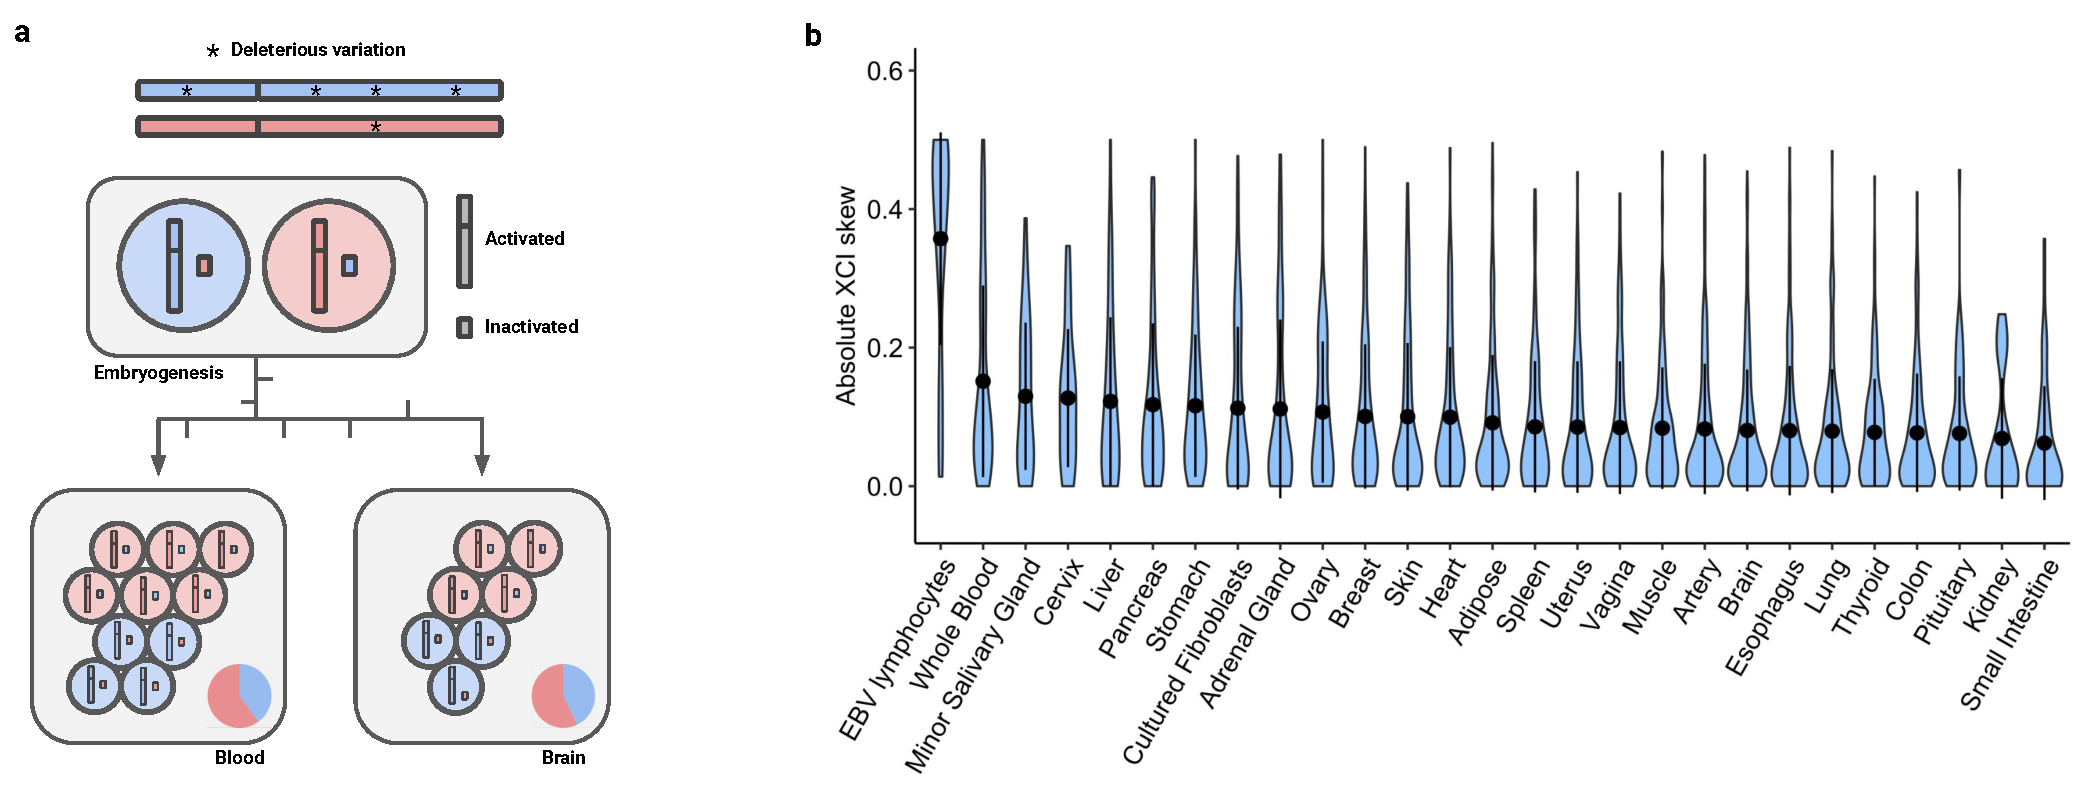
\includegraphics[width=\textwidth]{chapter4/Figures/Figure_1.pdf}
    \caption{
        Measuring XCI skew across tissues 
        \textbf{a}, Schematic overview of selection hypothesis. An individual inherits one haplotype (red) that is more fit than the other (blue) due to genetic variation. Given equal population sizes in embryonic development, we hypothesize that fitness differences will produce skewed populations in fully developed tissues.
        \textbf{b}, Violin plot of absolute XCI skew on the y-axis. Tissues are sorted by mean on the x-axis. Dots indicate mean of the absolute skew with vertical lines indicating one standard deviation.}
    \label{fig:fig4.1}
\end{figure}
\section{Methods}
\subsection{Transcriptomic and genetic data}

The following data were processed and made available by the GTEx consortium \cite{GTEx_Consortium2020-xx}. GENCODE v26 and the GRCh38 human reference genome was used to process both WGS and RNA-seq data. RNA-seq data was aligned using STAR with WASP filtering. Allele-specific read counts at heterozygous sites were quantified with GATK ASEReadCounter. Genetic variants were called from whole genome sequencing data and phased with read-aware SHAPEIT2. All analyses were restricted to caucasian samples. 

\subsection{Quantifying XCI skew}

Allele-specific read counts were matched to haplotypes from the phased WGS data. Only heterozygous sites within fully inactivated genes reported by Carrel and Willard \cite{Carrel2005-zm} and Cotton et al \cite{Cotton2013-jl} were considered. We further selected genes where no females were observed to escape inactivation in Cotton et al. This filtering yielded heterozygous sites within 117 genes considered to be fully inactivated. LiftOver (https://genome.ucsc.edu/cgi-bin/hgLiftOver) was used to convert these reported gene windows from GRCh37 to GRCh38 positions. Moreover, we only considered variants that had at least 10 overlapping reads. XCI skew was calculated at each heterozygous site in the gene windows as the number of reads coming from one haplotype divided by the total number of reads at the site. The final XCI skew measurement for each sample was the median of these per-site observations as done in previous work \cite{Shvetsova2019-re}. The haplotypes were arbitrarily labeled as H1 and H2, and skew was calculated as the number of reads mapping to H1 divided by the total reads at each site. Since haplotypes are not readily distinguishable as maternal or paternal, we also calculated the absolute XCI skew as the absolute deviation of this value from 0.5. Correlation between skewing in tissues was calculated as the Pearson correlation of pairwise-complete observations between tissue pairs where 25 or more individuals had both tissues sampled. 

We also calculated skew in the same manner in autosomes. Specifically, if $m$ heterozygous sites were used to calculate XCI in a sample, we randomly selected $m$ heterozygous sites with at least 10 overlapping RNA-seq reads on the q-arm of each non-acrocentric autosome. We used these sites to calculate skew for each autosome as the median value. Since extreme XCI skewing was observed in EBV-transformed lymphocytes, we removed these samples from all downstream analyses for both X and autosomal chromosomes. 

\subsection{Genetic score association}

Four scores were defined to measure genetic burden of X chromosome haplotypes in females. Each score was calculated using SNPs and indels in the SHAPEIT2 phased VCF files provided by GTEx \cite{GTEx_Consortium2020-xx}. Each score was calculated using all heterozygous variants with physical positions that did not fall within the 117 genomic windows corresponding to fully inactivated genes used to calculate skew. First, we considered the difference in average SNP CADD score \cite{Rentzsch2019-pk} between the two haplotypes. A higher CADD score corresponds to an increased likelihood of deleteriousness. CADD Phred scores for SNPs were retrieved using VEP \cite{McLaren2016-jd}. The CADD score associated with all alternate SNP alleles occuring on a haplotype was averaged. CADD burden scores were defined as the average CADD score of haplotype H1 subtracted from the average CADD score of haplotype H2. 

The remaining scores were proportions of different types of mutations carried by the H1 haplotype. We considered the proportion of alternate alleles (both SNPs and indels), missense SNPs, and synonymous SNPs carried by a haplotype. This proportion is calculated as the count of the variant-type on haplotype H1 divided by the total number of these variants found across both haplotypes. Annotations indicating the coding consequence of variants were obtained using VEP. 

We associated these scores with XCI skew using a linear mixed model. Specifically, we used the lmer function from the lmerTest package \cite{Kuznetsova2017-jp} to fit the following model across all tissues, where the (1\textbar Grouping) notation indicates a random intercept for the specified grouping:
\begin{equation}
\text{H1 XCI Skew} \sim \text{H1 Burden + Age + (1\textbar Individual) + (1\textbar Tissue)}
\end{equation}
In this model, we include random intercepts for the individual and tissue of origin for each sample. The significance of these associations were determined using a one-sided t-test, under the assumption that increased burden will decrease skewing towards a haplotype. The p-values were calculated as the value of the cumulative density function of the t-distribution given the t-values and degrees of freedom returned by the lmer function. 

Blood-related polygenic scores were retrieved from PGS Catalog \cite{Lambert2021-iu}. We used scores for the following cell counts: platelet (PGS000186), red blood cell (PGS000187), basophil (PGS000163), neutrophil (PGS000182), eosinophil (PGS000165), monocyte (PGS000177), and lymphocyte (PGS000172) \cite{Vuckovic2020-gf}. GRCh38 positions of the variants used for these scores were retrieved from SNP Nexus \cite{Oscanoa2020-ac}. We calculated each polygenic score for both haplotypes as the linear combination of the score weights and the corresponding effect alleles if they occur on the haplotype. We modeled the difference in polygenic scores as follows:
\begin{equation}
\text{H1 XCI Skew} \sim \text{(H1 PGS - H2 PGS) + Age + (1\textbar Individual) + (1\textbar Tissue)}
\end{equation}

The significance of these associations were determined by using a one-sided t-test, under the assumption that increased proliferative potential will increase skewing towards a haplotype. Specifically, p-values were calculated by subtracting the cumulative density function of the t-distribution given the t-values and degrees of freedom from one. 

Each of the scores described above were calculated for autosomal haplotypes using variants that occur on the p-arm of each non-acrocentric chromosome. As controls, we repeated the association tests for these autosomes with the following model:
\begin{align}
\begin{split}
\text{H1 XCI Skew} \sim & \text{ (H1 PGS - H2 PGS) + Age +} \\
                        & \text{ (1\textbar Individual) + (1\textbar Tissue) + (1\textbar Chromosome)}
\end{split}
\end{align}
where “H1 score” refers to the burden and proliferation polygenic scores defined above and “Chromosome” refers to the autosome used to generate the sample. A Bonferroni-corrected significance threshold of 0.05/8 was used for the 4 burden scores and 0.05/14 was used for the 7 blood-related polygenic scores. 

\subsection{Identifying significant XCI loci}

The phased X chromosome variants were filtered with PLINK 2 \cite{PLINK2}. SNPs were extracted with a minor allele frequency threshold of 0.01 and Hardy-Weinberg equilibrium p-value threshold of 1e-6. LD pruning was performed with a window size of 100 kilobases, step size of 5 variants, and $r^2$ threshold of 0.5. 

These filtered variants were marginally tested in a linear mixed model to measure association with absolute XCI skew. We fit the following linear mixed model:
\begin{equation}
\text{Absolute XCI Skew} \sim \text{Heterozygous + Age + (1\textbar Individual) + (1\textbar Tissue)}
\end{equation}
where Heterozygous is 1 if the sample is heterozygous for the variant and 0 if the sample is homozygous. We modeled absolute skewing under the assumption that heterozygosity will lead to differences in fitness and consequently increased overall skewing. Given this assumption, we determined the significance of these associations using a one-sided t-test under this hypothesis of a positive effect size if one exists. The resulting p-values were converted to q-values \cite{Storey2003-kx} and considered significant using a threshold corresponding to a 0.05 local false discovery rate.

At the two significant loci, this linear mixed model was also used to determine the significance of the difference in skewing between homozygous samples and groups defined by the phasing of the variant in heterozygous individuals. For these associations, we fit the following model separately for individuals with the variant on H1 and on H2:
\begin{equation}
\text{H1 XCI Skew} \sim \text{Heterozygous + Age + (1\textbar Individual) + (1\textbar Tissue)}
\end{equation}
Since we do not assume the direction of individual variant effects on XCI skewing, we performed a two-sided t-test to determine significance of these associations. 

\subsection{Associating XCI-linked genetics in males}

To address the possibility that the burden and proliferation scores are capturing regulatory effects, such as downregulation of a haplotype rather than increased inactivation, we calculated these scores within males. Like in the female samples, we utilized variants with physical positions that did not fall within the windows of the 117 fully inactivated genes used to calculate skew.  For each individual, only variants reported as homozygous in the VCF files were considered, since heterozygous calls should not occur in the males with one X chromosome. Given that males have one X chromosome, we associated these scores with the expression of each gene on the X chromosome. We fit a model similar to those used for identifying expression quantitative trait loci. Specifically, we performed a linear regression within each tissue independently, correcting for the top 5 genetic principal components, PCR, and platform. We also corrected for PEER factors \cite{Stegle2012-uf}, using 15 factors for sample sizes less than 150 and adding an additional 15 factors for each 100 samples. The resulting p-values from the linear regression across all tissues were converted to q-values and considered significant at a local false discovery rate threshold of 0.05. 

\section{Results}

\subsection{Estimating XCI skew from RNA-seq data}

We analyzed data generated by the GTEx consortium \cite{GTEx_Consortium2020-xx}, which included RNA-seq and phased whole genome sequencing data measured across 243 caucasian female samples and 472 caucasian male samples. We measured XCI skew in females as the difference in expression measured from each X chromosome in an RNA-seq experiment. Since XCI does not completely silence the entire X chromosome, we restricted our analysis to genes that have been previously observed to be fully inactivated \cite{Carrel2005-zm,Cotton2013-jl,Tukiainen2017-xm}. Read counts at heterozygous sites in these regions were assigned to haplotypes determined with phased whole genome sequencing data. The skew in RNA-seq reads was calculated at each site as the number of reads coming from one haplotype divided by the total number of reads. XCI skew for a sample was calculated as the median of these values as done by previous work \cite{Shvetsova2019-re}. A median of 45 heterozygous sites were used for this calculation across the samples (Figure \ref{fig:supp_fig4.1}). We observed variability in XCI skew across tissues, with EBV-transformed lymphocytes exhibiting nearly complete skew in many samples (Figure \ref{fig:fig4.1}b).  Given this extreme skewing likely due to culture conditions, we removed these samples from downstream analyses. Furthermore, we observed correlation of XCI skew across the different tissues (Figure \ref{fig:supp_fig4.2}).

\begin{figure}[ht]
    \centering
    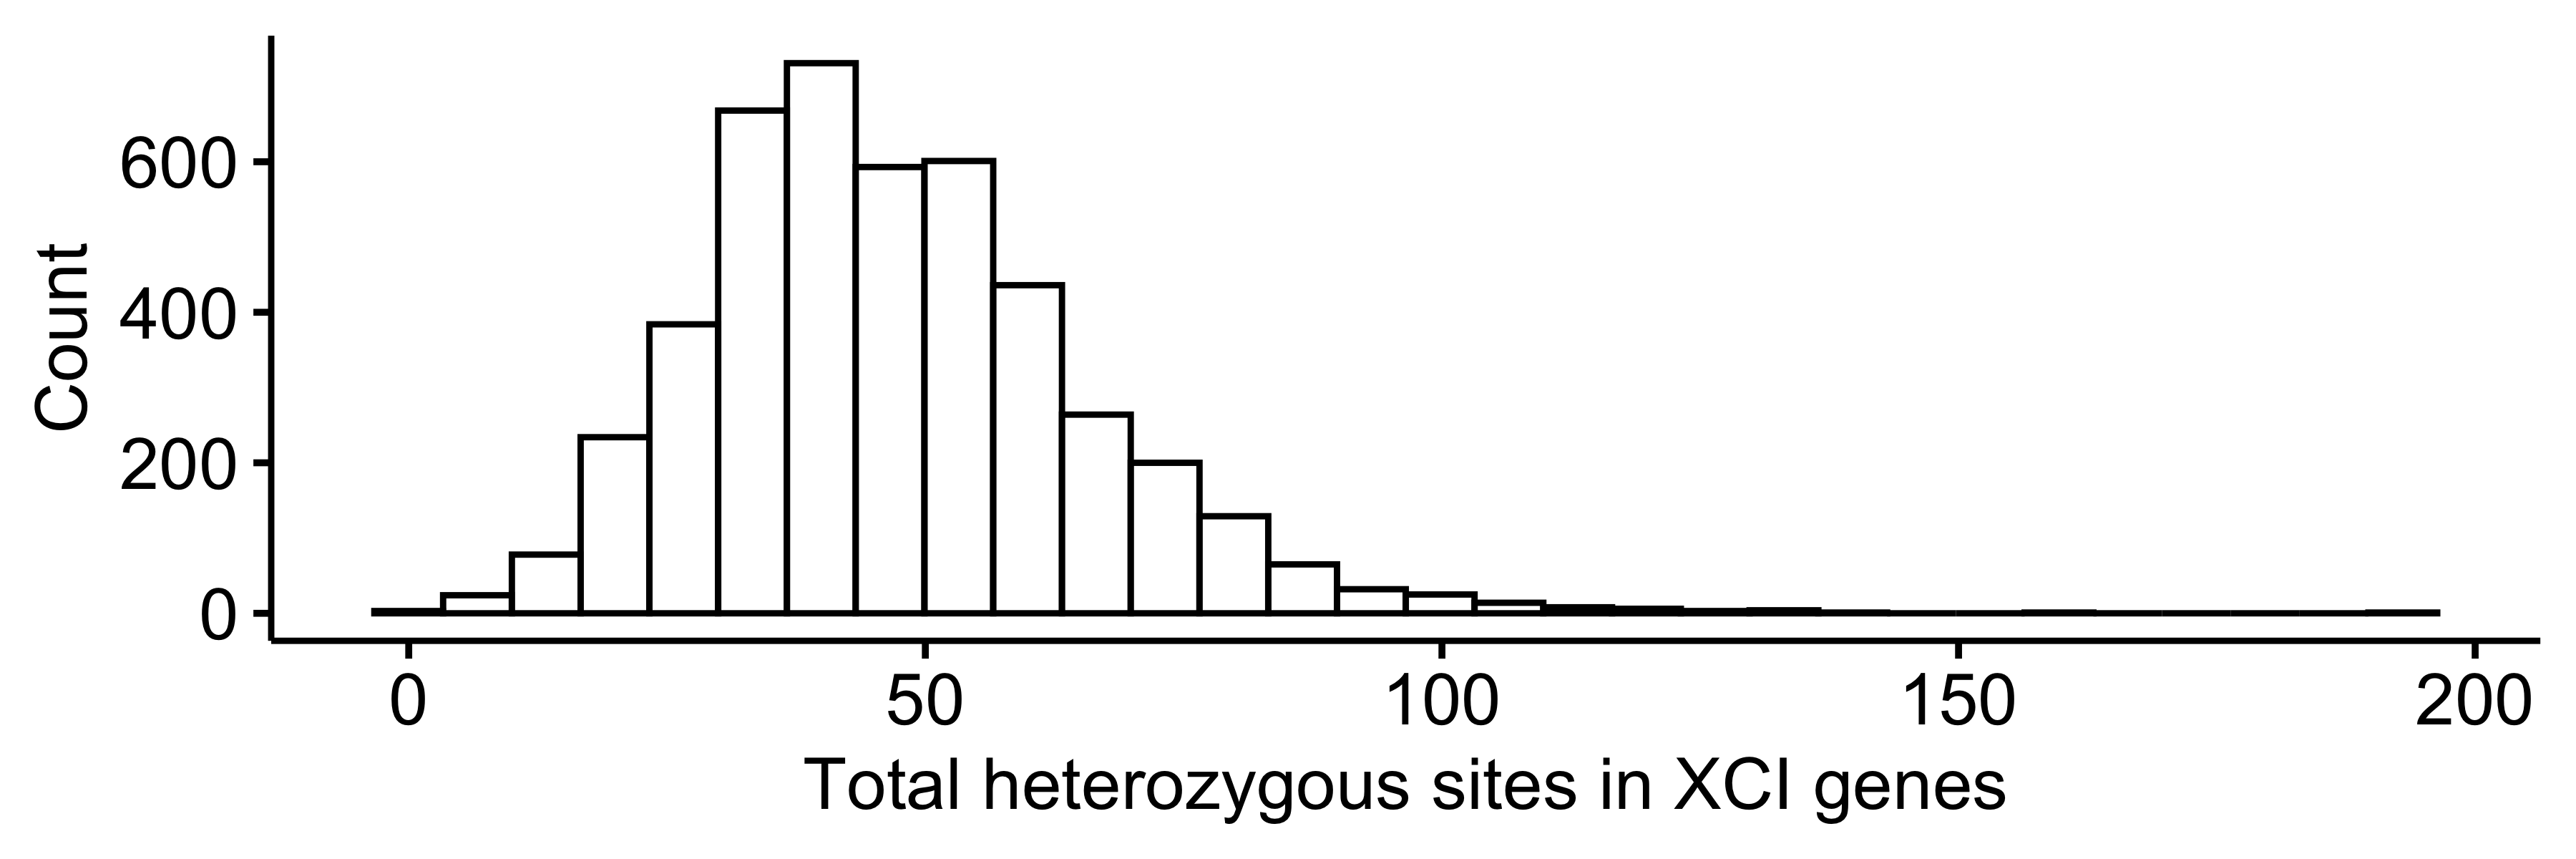
\includegraphics[width=0.75\textwidth]{chapter4/Figures/Supplementary_Figure_1.png}
    \caption{
        Histogram of number of heterozygous sites with coverage of 10 or more RNA-seq reads and within fully inactivated genes used to calculate XCI skew for each sample. We observed a mean of 46.805 and median of 45 variants used to calculate skew (the median of per-site skew). 
    }
    \label{fig:supp_fig4.1}
\end{figure}
\begin{figure}[ht!]
    \centering
    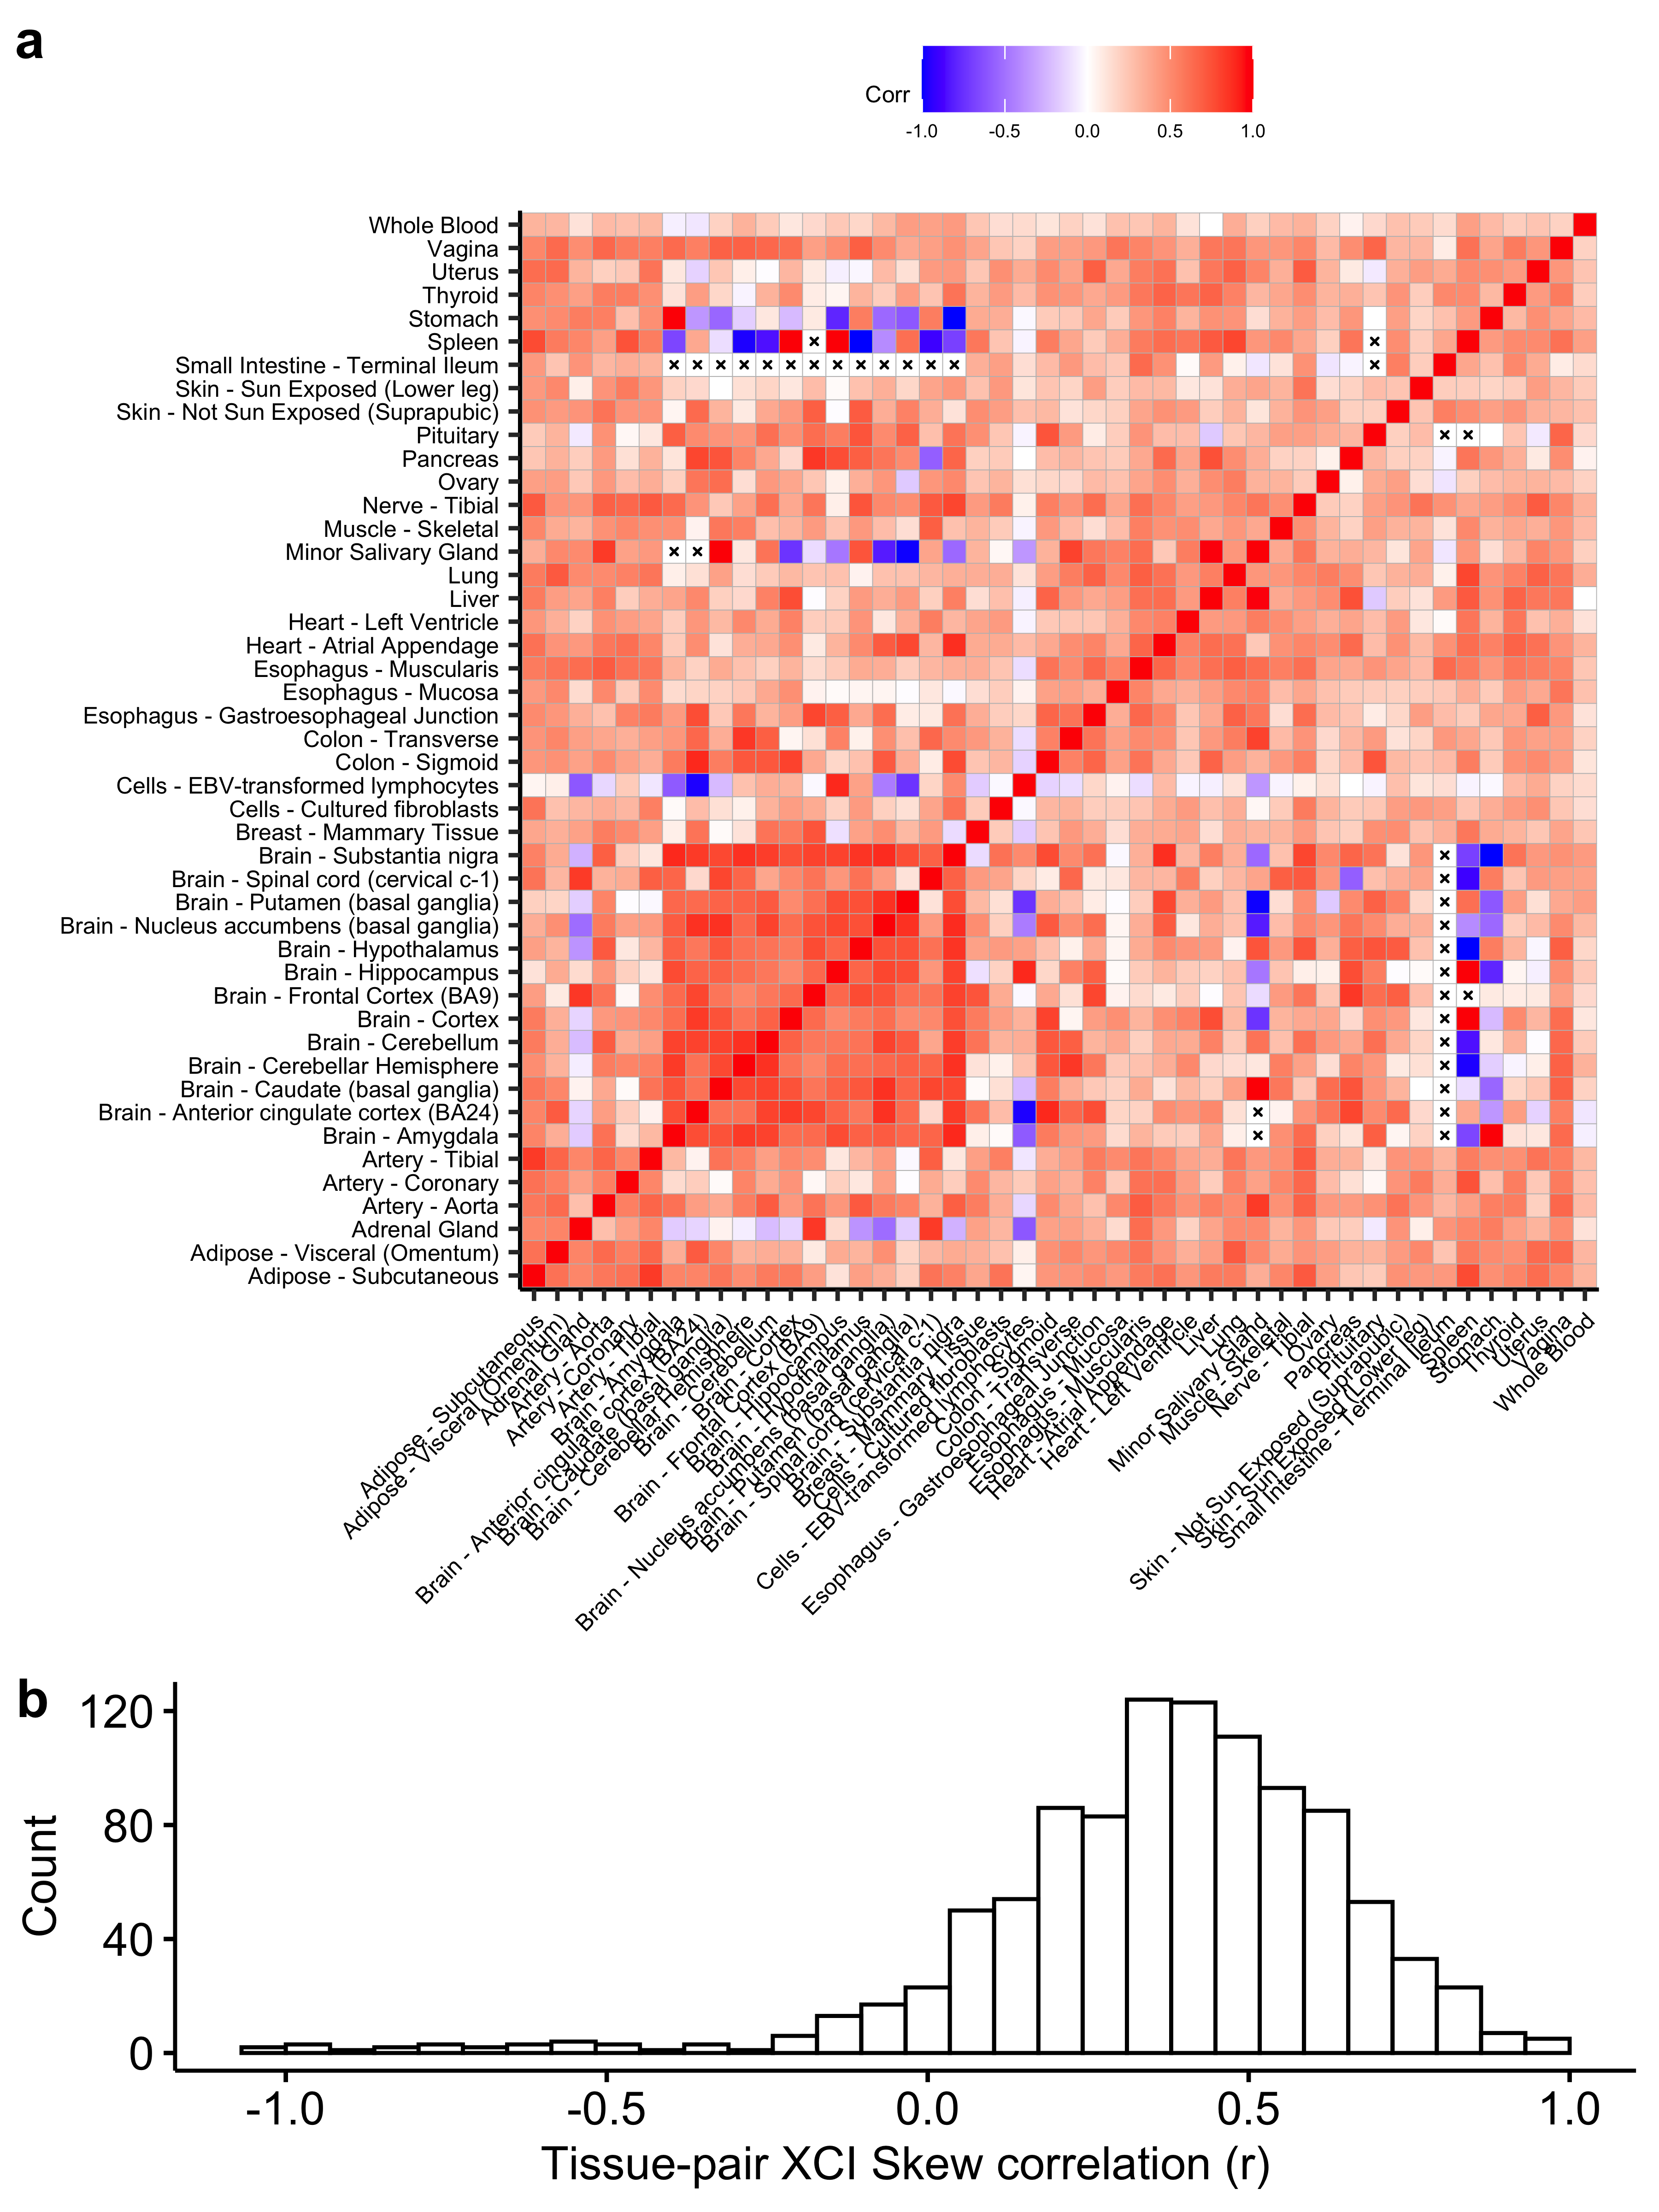
\includegraphics[width=0.75\textwidth]{chapter4/Figures/Supplementary_Figure_2.png}
    \caption{
        Pearson correlation of XCI skew between tissues.
        \textbf{a}, Correlation matrix of tissue-specific XCI skew. White boxes with 'X' symbol indicate that less than 25 observations were available for the tissue pair.
        \textbf{b}, Histogram of correlation between 1,017 non-identical tissue pairs. We observed a mean correlation of 0.3663 and median of 0.3992.
    }
    \label{fig:supp_fig4.2}
\end{figure}

Inferring XCI skew from expression data can be confounded by both technological and biological factors that may lead to similar associations with our genetic burden scores. Reference bias, the tendency for RNA-seq reads with reference alleles to better map to a reference genome than non-reference alleles \cite{Stevenson2013-cg}, may be a significant confounding variable. This bias is especially relevant to the genetic burden defined by the proportion of alternate alleles carried by a haplotype. For example, an alternate allele may have lower observed expression than the reference allele simply due to reference bias rather than XCI skew. To account for this source of bias, we utilized RNA-seq reads that were aligned with a filter utilizing WASP, a method that accounts for reference bias by mapping reads with swapped genotypes \cite{Van_de_Geijn2015-oy}.
Regulatory effects of genetic variation may also lead to imbalances in expression \cite{Castel2018-wo} measured from each X chromosome that may be erroneously attributed to skew in X chromosome inactivation. To address this source of confounding, we performed similar experiments using the non-acrocentric autosomes (chromosomes with arms of roughly equal size) of the female samples. In short, we calculated skewing at heterozygous sites that were captured by RNA-seq reads on the q or long arm of the autosome. We observed no significant level of average ‘skewing’ in these chromosomes (Figure \ref{fig:supp_fig4.3}). 

\begin{figure}[ht]
    \centering
    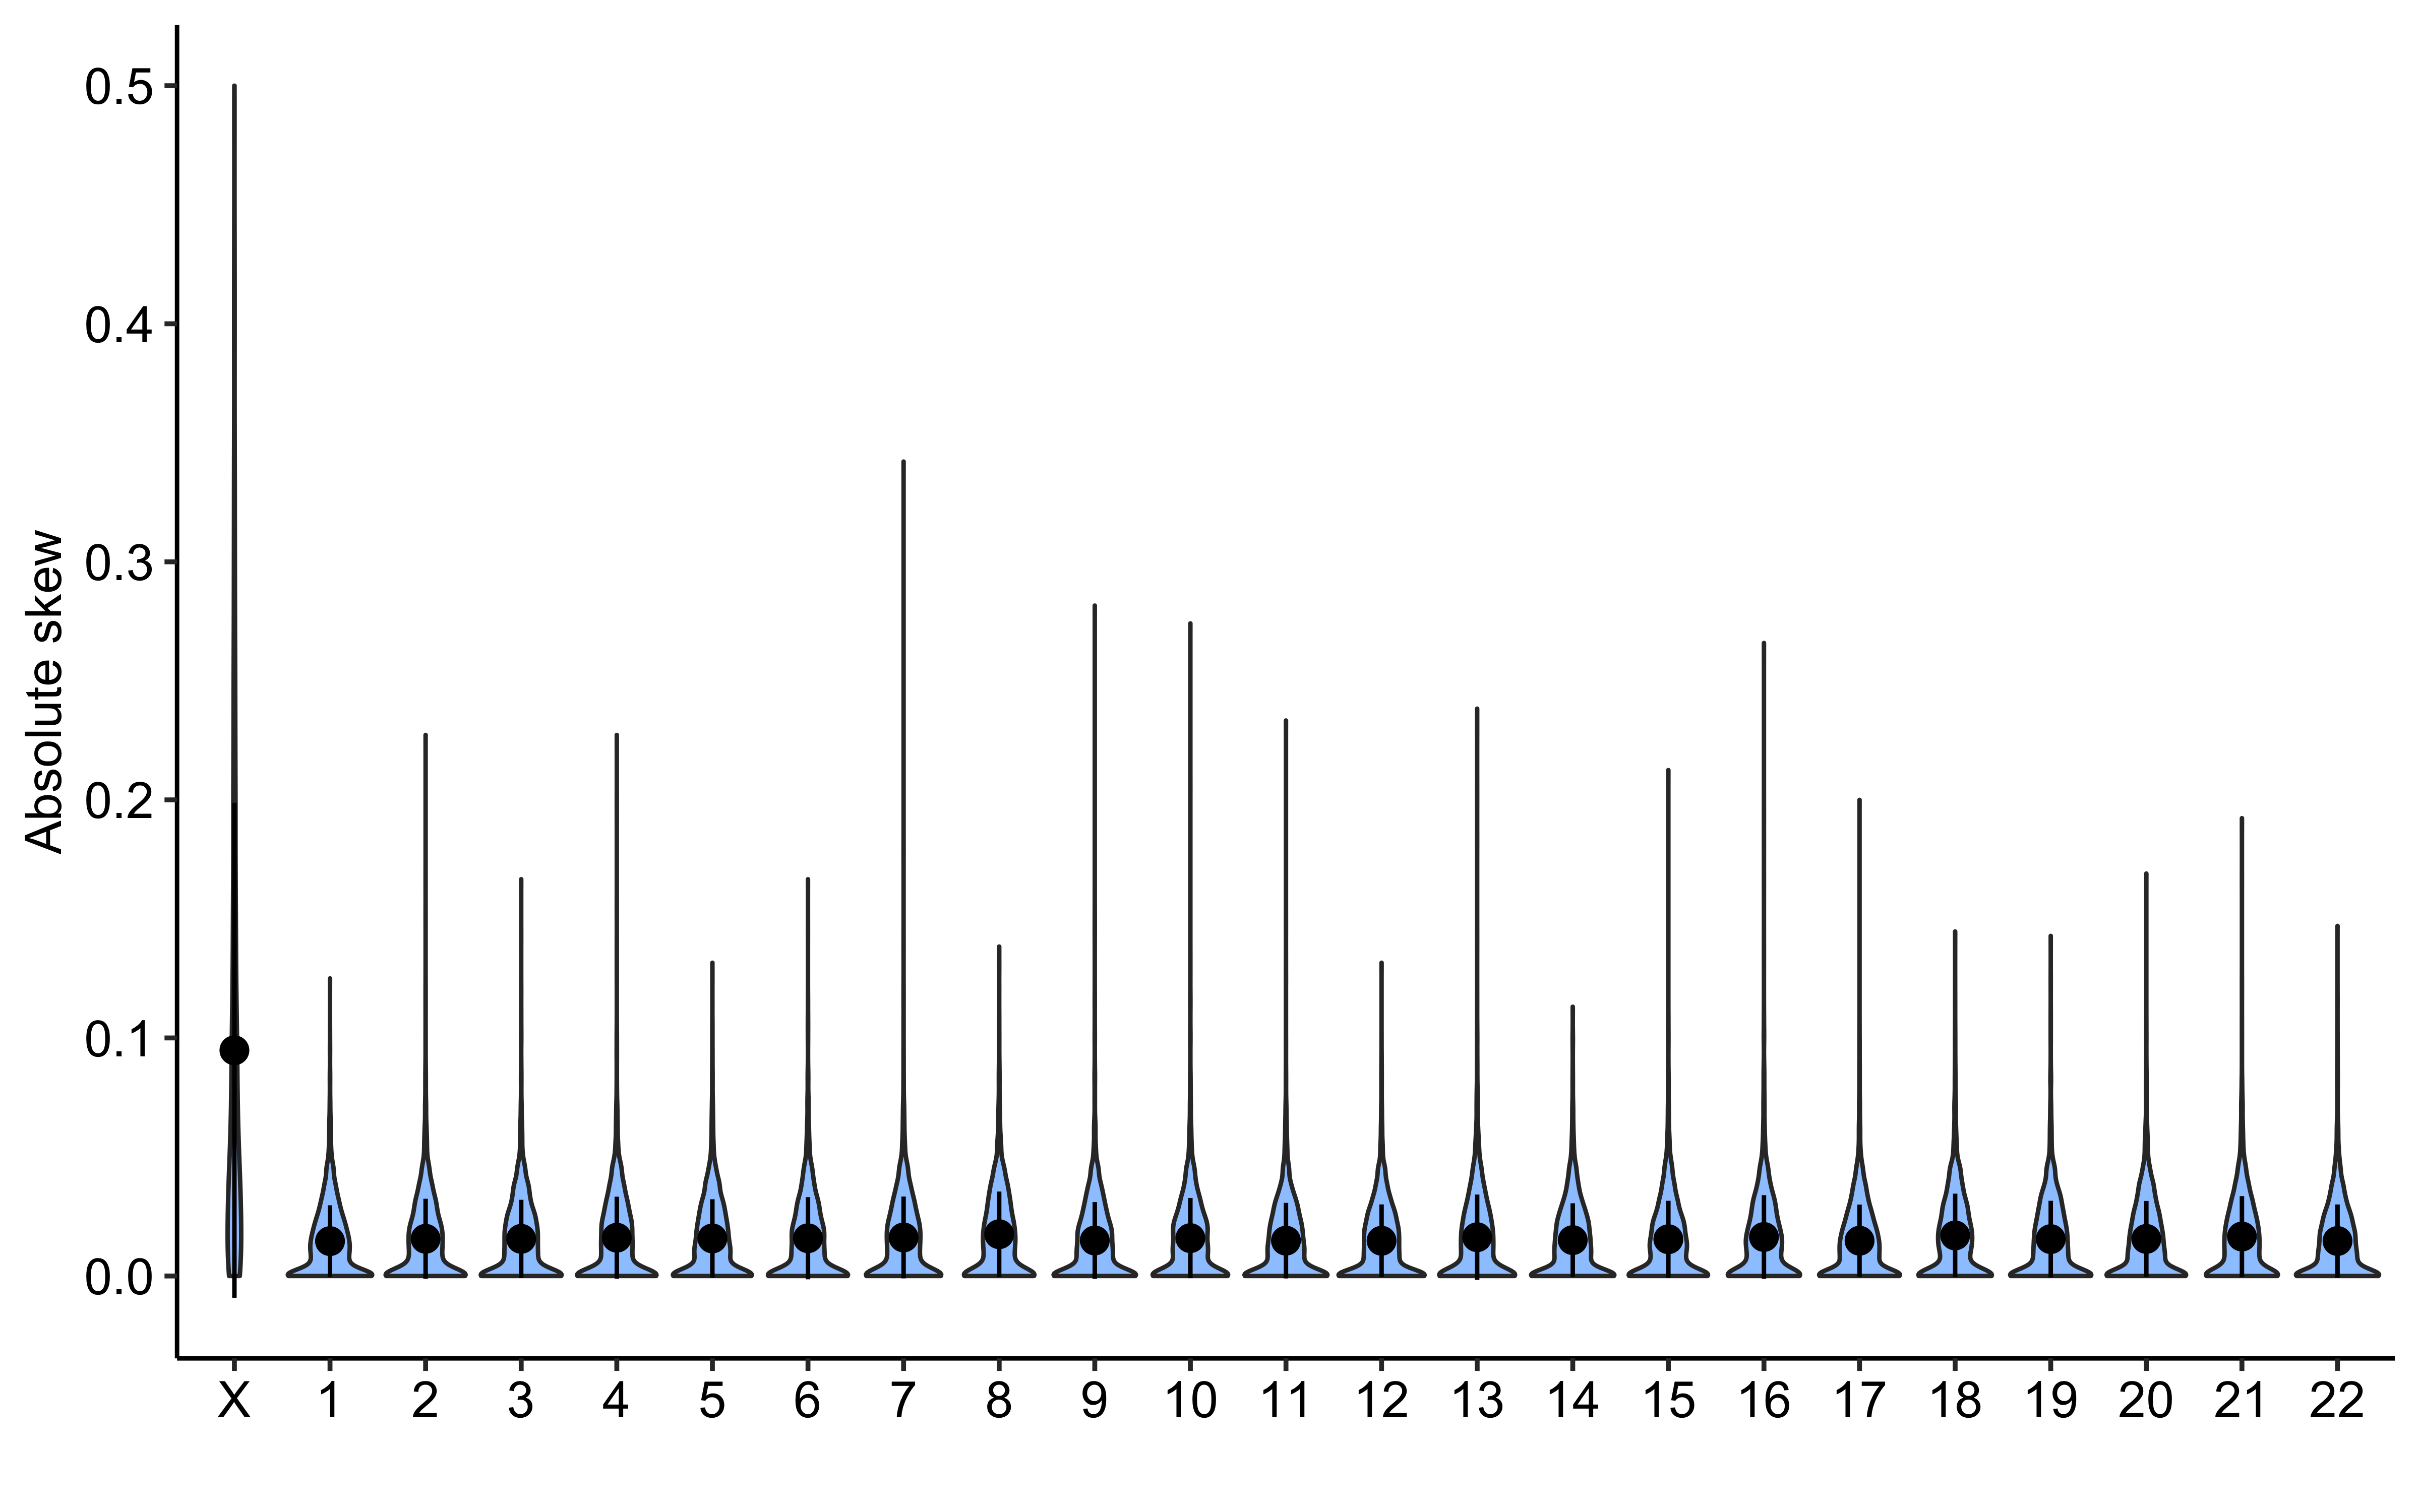
\includegraphics[width=0.75\textwidth]{chapter4/Figures/Supplementary_Figure_3.png}
    \caption{
        Estimated absolute skew in expression at heterozygous sites on the X chromosome and non-acrocentric autosomes. On the X chromosome, this value is used as the estimate of inactivation skewing since heterozygous sites are within fully inactivated genes. On the autosomes, an equal number of heterozygous sites used on the X chromosome for each sample were randomly selected from the q-arm to estimate the median skew in expression. Dots indicate mean of absolute skew with vertical lines indicating one standard deviation.
    }
    \label{fig:supp_fig4.3}
\end{figure}

We also performed an analysis of the male GTEx samples to test the possibility of regulatory effects rather than skewing in inactivation. Since males only have one X chromosome, we associated genetic features with expression of each gene on the X chromosome. If our genetic scores are associated with downregulation of expression rather than XCI skew, we anticipated this experiment to show a significant negative association with the expression of X chromosome genes across males.

\subsection{Genetic burden is associated with XCI skew}

We defined the following genetic burden scores for this analysis: the proportion of missense and synonymous mutations carried by each haplotype, and the difference in average CADD score \cite{Rentzsch2019-pk} between the two haplotypes. CADD scores provide a quantitative measure of the predicted deleteriousness of a variant. Only genetic variation with genomic positions outside of the gene windows that were used to calculate XCI skew were considered in these scores to avoid capturing cis regulatory effects. To associate these burden measures with XCI skew, we fit a linear mixed model with random intercepts accounting for the individual of origin for each tissue sample and tissue type. In this model, the difference in CADD score between haplotypes had a significant negative effect on XCI skew (coefficient = -0.1289 ± 0.0451, p = 0.0023) (Figure \ref{fig:fig4.2}a). This result suggests that a higher genetic burden in terms of deleterious variation is associated with higher rates of inactivation of the haplotype. We found that this association was not significant across the non-acrocentric autosomes (Table \ref{table:table4.1}). In addition, these burden scores were not associated with the regulation of gene expression on the X chromosome in male samples. 

\begin{figure}[ht]
    \centering
    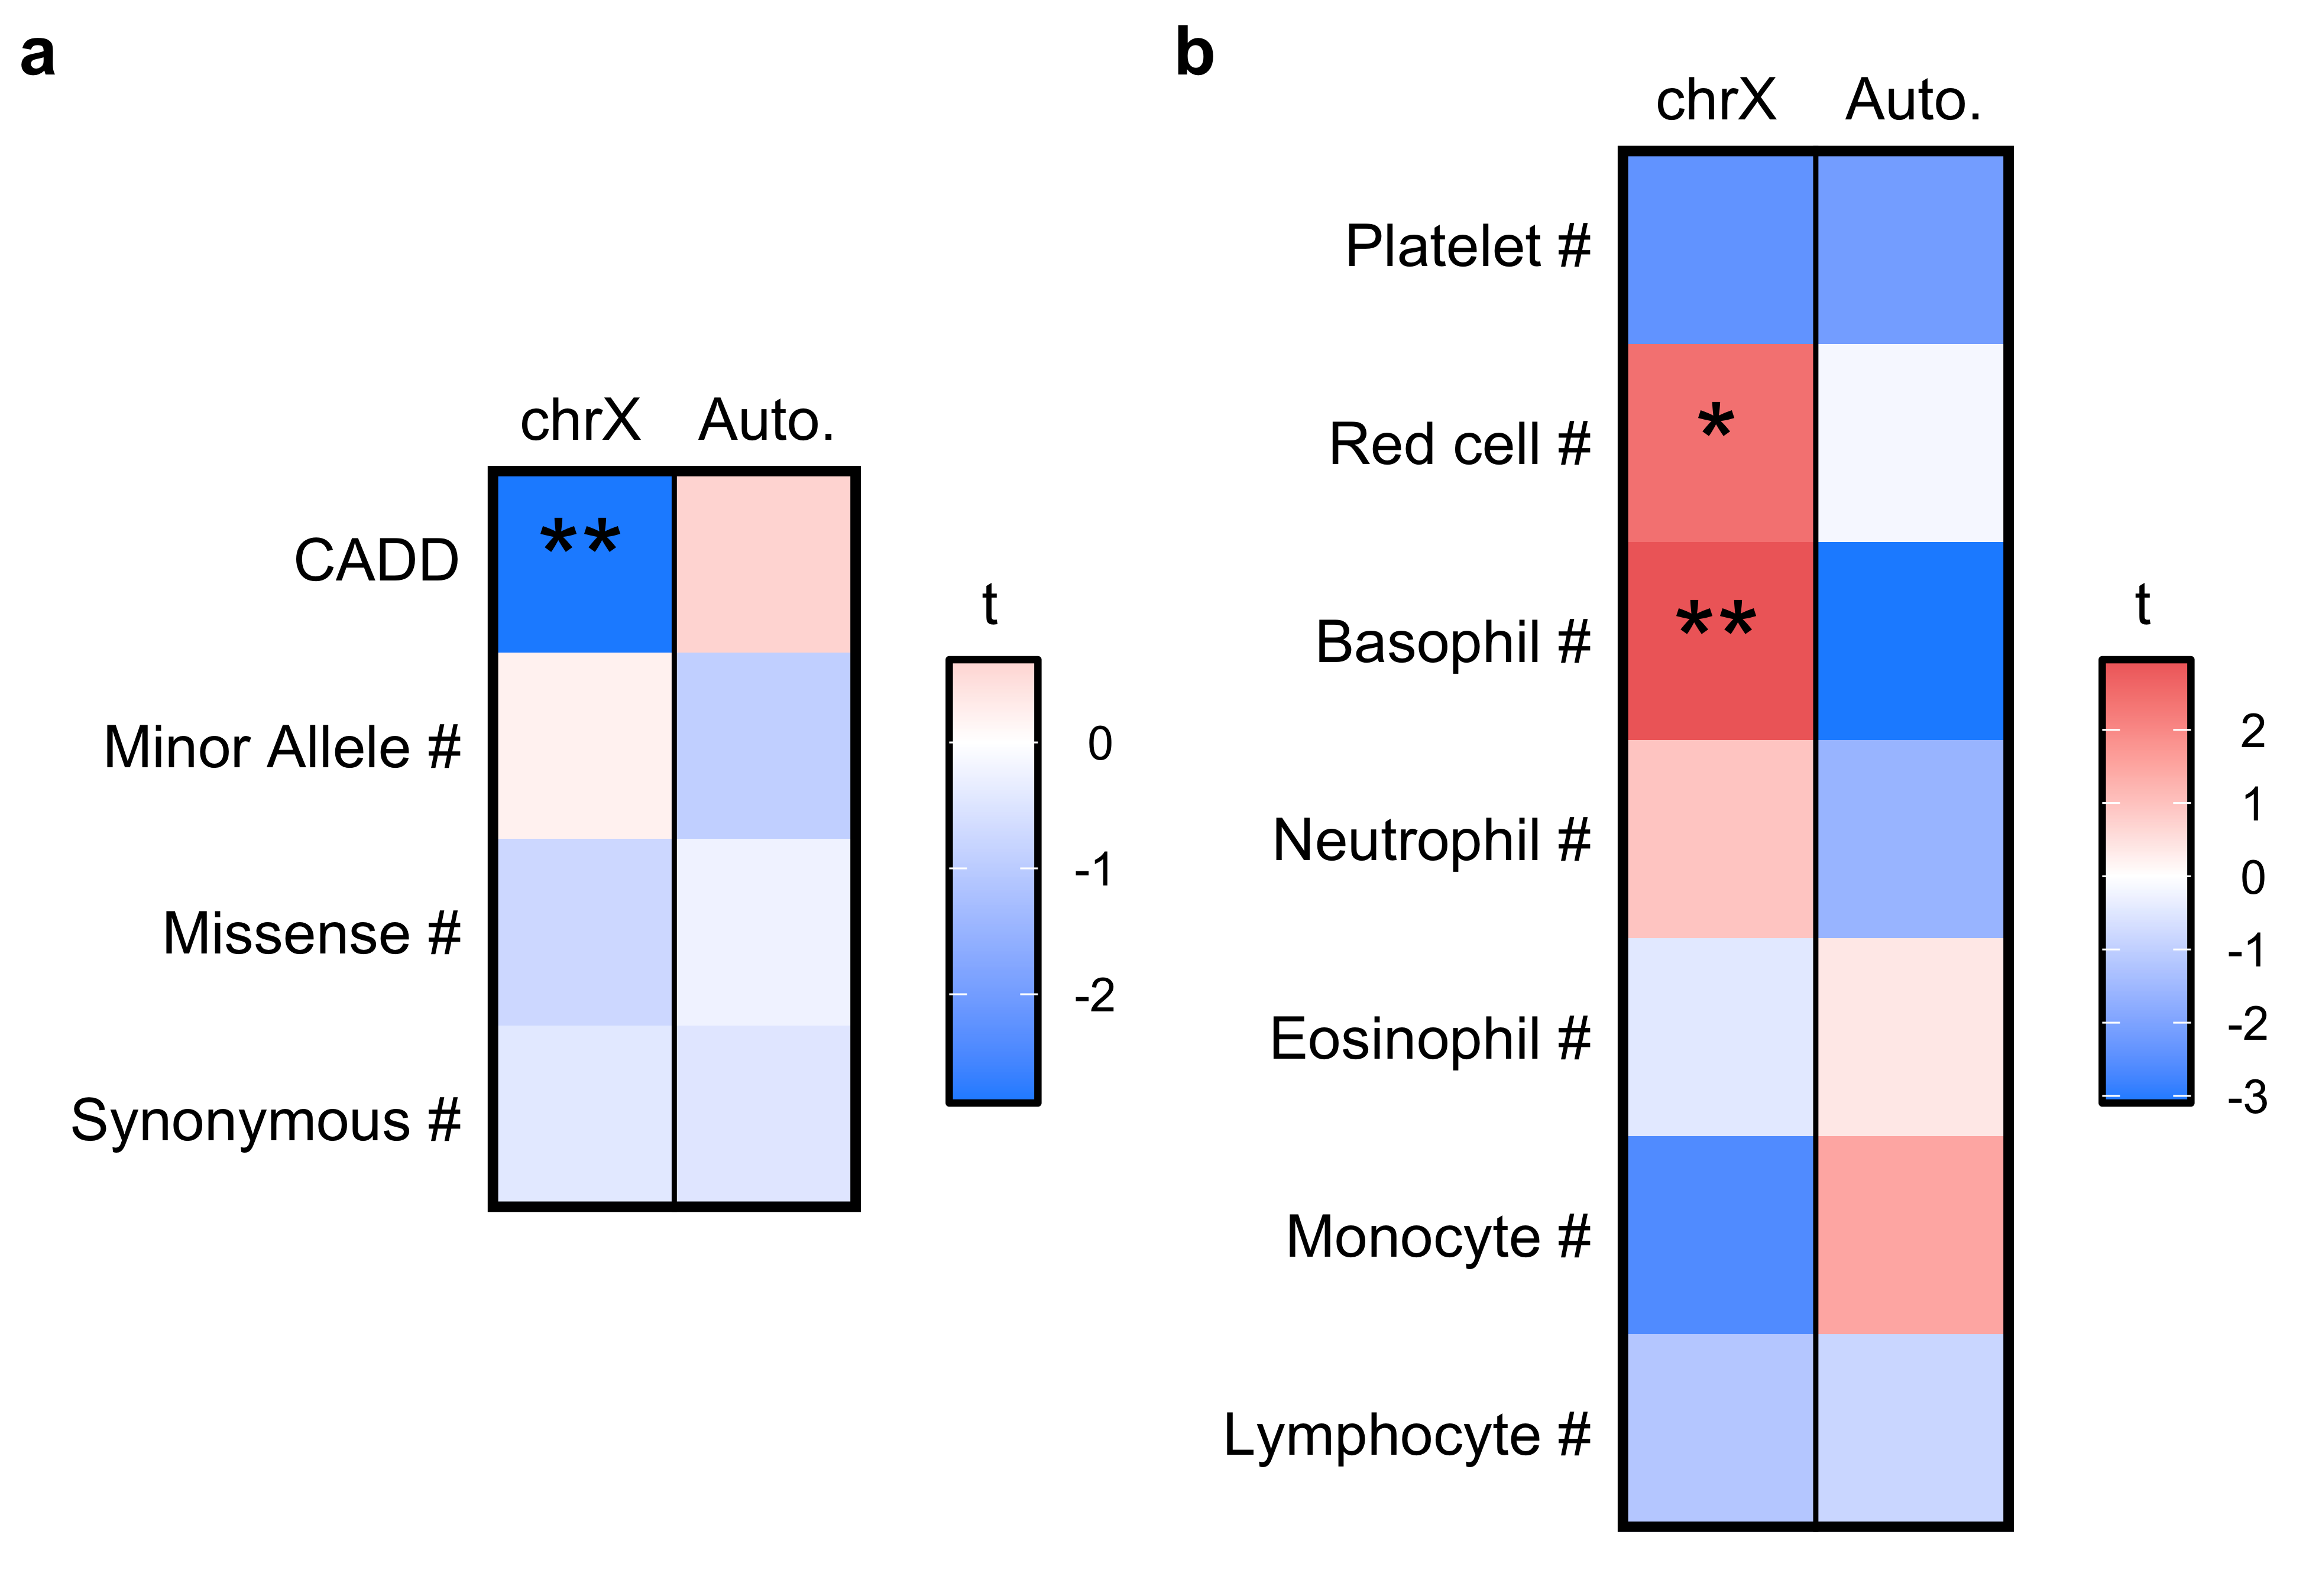
\includegraphics[width=0.5\textwidth]{chapter4/Figures/Figure_2.png}
    \caption{
        Association between genetic scores and skew estimated from expression at heterozygous sites on X chromosome (chrX) and non-acrocentric autosomes (Auto.). Colors indicate the relative t-score from a linear mixed model association test with an asterisks (*) indicating significance at $\alpha=0.05$ and double asterisks (**) indicating significance after Bonferroni correction.
        \textbf{a}, Association results of genetic burden scores with estimated skew. A one-sided t-test was performed under the assumption that increased genetic burden decreases skew towards the haplotype. CADD indicates difference in mean CADD score of each haplotype. The remaining scores compare the number of the indicated mutations on each haplotype.
        \textbf{b}, Association results of proliferative polygenic scores with estimated skew. Counts of different blood cell types were used as a proxy for proliferative potential. A one-sided t-test was performed under the assumption that increased proliferation genetic scores will increase skew towards the haplotype.}
    \label{fig:fig4.2}
\end{figure}
\begin{table}[ht]
\scriptsize
\caption{Burden associations with skewing in XCI and autosomal q-arm expression}
\centering
\begin{tabular}{llllll}
  \hline
 Burden Score & Chromosome(s) & $\beta$ (s.e.) & df & $t$ & $P$ \\ 
  \hline
CADD & chrX & -0.1289 (0.0451) & 240.6684 & -2.8579 & 0.0023 \\ 
   & Auto. & 0.0024 (0.0037) & 60762.2663 & 0.6516 & 0.7427 \\ 
  Minor Allele \# & chrX & 0.0097 (0.0453) & 240.5593 & 0.2141 & 0.5847 \\ 
   & Auto. & -0.0034 (0.0037) & 58076.8103 & -0.9263 & 0.1772 \\ 
  Missense \# & chrX & -0.0355 (0.0476) & 238.7277 & -0.7452 & 0.2285 \\ 
   & Auto. & -0.0009 (0.0037) & 59330.7798 & -0.2314 & 0.4085 \\ 
  Synonymous \# & chrX & -0.0202 (0.0463) & 239.3741 & -0.4356 & 0.3318 \\ 
   & Auto. & -0.0018 (0.0037) & 39637.5931 & -0.4748 & 0.3175 \\ 
   \hline
\end{tabular}
\label{table:table4.1}
\end{table}

\subsection{Variation in proliferation-related polygenic scores is associated with XCI Skew}

We utilized publicly available polygenic risk score weights to calculate the proliferative potential of each haplotype in the female samples. Specifically, we used various blood cell counts as phenotypes under the assumption that these scores are concordant with hematopoiesis and proliferative cell activity \cite{Loh2020-mb}. We found that the haplotype with the higher red blood cell polygenic score (coefficient = 0.1116 ± 0.0462, p = 0.0082) and basophil polygenic score (coefficient = 0.1355 ± 0.0460, p = 0.0018) tends to be overrepresented in terms of XCI skewing (Figure \ref{fig:fig4.2}b). These results imply that higher proliferative-related polygenic scores are associated with an enrichment for cells with this haplotype active across tissues. We also ran similar autosomal and male analyses to test the alternative hypothesis that these polygenic scores may be capturing gene regulatory effects. We found no significant associations between these scores in the female non-acrocentric autosomes (Table \ref{table:table4.2}). In the analysis of male samples, the basophil polygenic score was significantly associated with increased expression of AFF2 in 4 tissues (Table \ref{table:table4.4}). However, this gene is considered a variable XCI escape gene and therefore was not used to calculate XCI skew in the female samples.

\begin{table}[ht]
\scriptsize
\caption{Proliferation-related polygenic score associations with skewing in XCI and autosomal q-arm expression}
\centering
\begin{tabular}{llllll}
  \hline
Polygenic Score & Chromosome(s) & $\beta$ (s.e.) & df & $t$ & $P$ \\ 
  \hline
Platelet \# & chrX & -0.1093 (0.0456) & 240.8663 & -2.3997 & 0.9914 \\ 
   & Auto. & -0.0079 (0.0037) & 58466.4918 & -2.1498 & 0.9842 \\ 
  Red cell \# & chrX & 0.1116 (0.0462) & 238.7682 & 2.4172 & 0.0082 \\ 
   & Auto. & -0.0006 (0.0037) & 54155.3786 & -0.1623 & 0.5645 \\ 
  Basophil \# & chrX & 0.1355 (0.0460) & 237.3432 & 2.9487 & 0.0018 \\ 
   & Auto. & -0.0113 (0.0037) & 60017.3402 & -3.0875 & 0.9990 \\ 
  Neutrophil \# & chrX & 0.0451 (0.0469) & 238.1159 & 0.9606 & 0.1689 \\ 
   & Auto. & -0.0059 (0.0037) & 57022.3082 & -1.6151 & 0.9469 \\ 
  Eosinophil \# & chrX & -0.0224 (0.0475) & 238.1788 & -0.4710 & 0.6810 \\ 
   & Auto. & 0.0014 (0.0037) & 60407.8660 & 0.3883 & 0.3489 \\ 
  Monocyte \# & chrX & -0.1209 (0.0463) & 237.1836 & -2.6126 & 0.9952 \\ 
   & Auto. & 0.0055 (0.0037) & 50177.1222 & 1.4848 & 0.0688 \\ 
  Lymphocyte \# & chrX & -0.0560 (0.0473) & 238.1101 & -1.1834 & 0.8811 \\ 
   & Auto. & -0.0031 (0.0037) & 57465.9629 & -0.8419 & 0.8001 \\ 
   \hline
\end{tabular}
\label{table:table4.2}
\end{table}


\begin{table}[ht]
\scriptsize
\caption{Covariates associated with chromosome X gene regulation in males.}
\centering
\begin{tabular}{lllllllll}
  \hline
 Covariate & Gene Name & Gene ID & XCI status & Tissue & $\beta$ (s.e.) & $P$ & $Q$ \\ %& $N$ \\ 
  \hline
  Basophil \# & AFF2 & ENSG00000155966.13 & Variable & Adipose (Subc.) & 0.1522 (0.0329) & 5.701e-06 & 0.0490 \\ % & 329 \\ 
  &  &  &  & Lung & 0.1825 (0.0374) & 1.841e-06 & 0.0317 \\ %& 302 \\ 
  &  & &  & Skin (Sup.) & 0.1616 (0.0344) & 4.353e-06 & 0.0490 \\ %& 297 \\ 
   &  &  &  & Thyroid & 0.1499 (0.0296) & 7.902e-07 & 0.0272 \\ %& 324 \\ 
  rs141680486 & TMEM187 & ENSG00000177854.7 & Inactive &  EBV lymphocytes & -0.3917 (0.0696) & 8.734e-07 & 0.0302 \\ %&  73 \\ 
   \hline
\end{tabular}
\label{table:table4.4}
\end{table}

\subsection{Variation in specific loci is significantly associated with XCI skew}

While the previous analyses suggest that genetic burden and proliferative potential is associated with skewed XCI, they do not provide specific variants or loci that contribute to this association. We performed an association study on the X chromosome to address this question. Specifically, we associated variants on the X chromosome with the absolute XCI skew measurements (Figure \ref{fig:fig4.3}a). We found 2 variants that were significant at a FDR of 0.05 (Table \ref{table:table4.3}). The first variant (rs141680486) is an intronic SNP found within the DMD gene, also known as dystrophin, and was significantly associated with increased absolute XCI skew (coefficient = 0.0203 ± 0.0041, p=7.978e-07). We observed large absolute skew in samples that were heterozygous for this variant compared to those who were homozygous (Figure \ref{fig:fig4.3}b). Moreover, we found that the haplotype with the minor allele tends to be more inactivated than the other haplotype in heterozygous samples (Figure \ref{fig:fig4.3}c). The second variant (rs73227260) is an intronic SNP in LOC101928359, a non-coding transcript,  and was also associated with increased absolute XCI skew (coefficient = 0.0199 ± 0.0041, p = 1.265e-06). We observed a high level of skewing in heterozygous individuals with no clear difference in directional skewing depending on the haplotype carrying the minor allele (Figure \ref{fig:supp_fig4.4}).

Since eQTLs may also cause skewing in expression within cells, we tested the association between these variants and gene expression on the X chromosome in males. We found that the DMD variant (rs141680486) is a significant eQTL for TMEM187 expression in EBV-transformed lymphocytes (coefficient = -0.3917 ± 0.0696, p=8.734e-07). However, we note that these lymphocyte samples were excluded from our female analyses due to extreme XCI skewing. 

\begin{figure}[ht!]
    \centering
    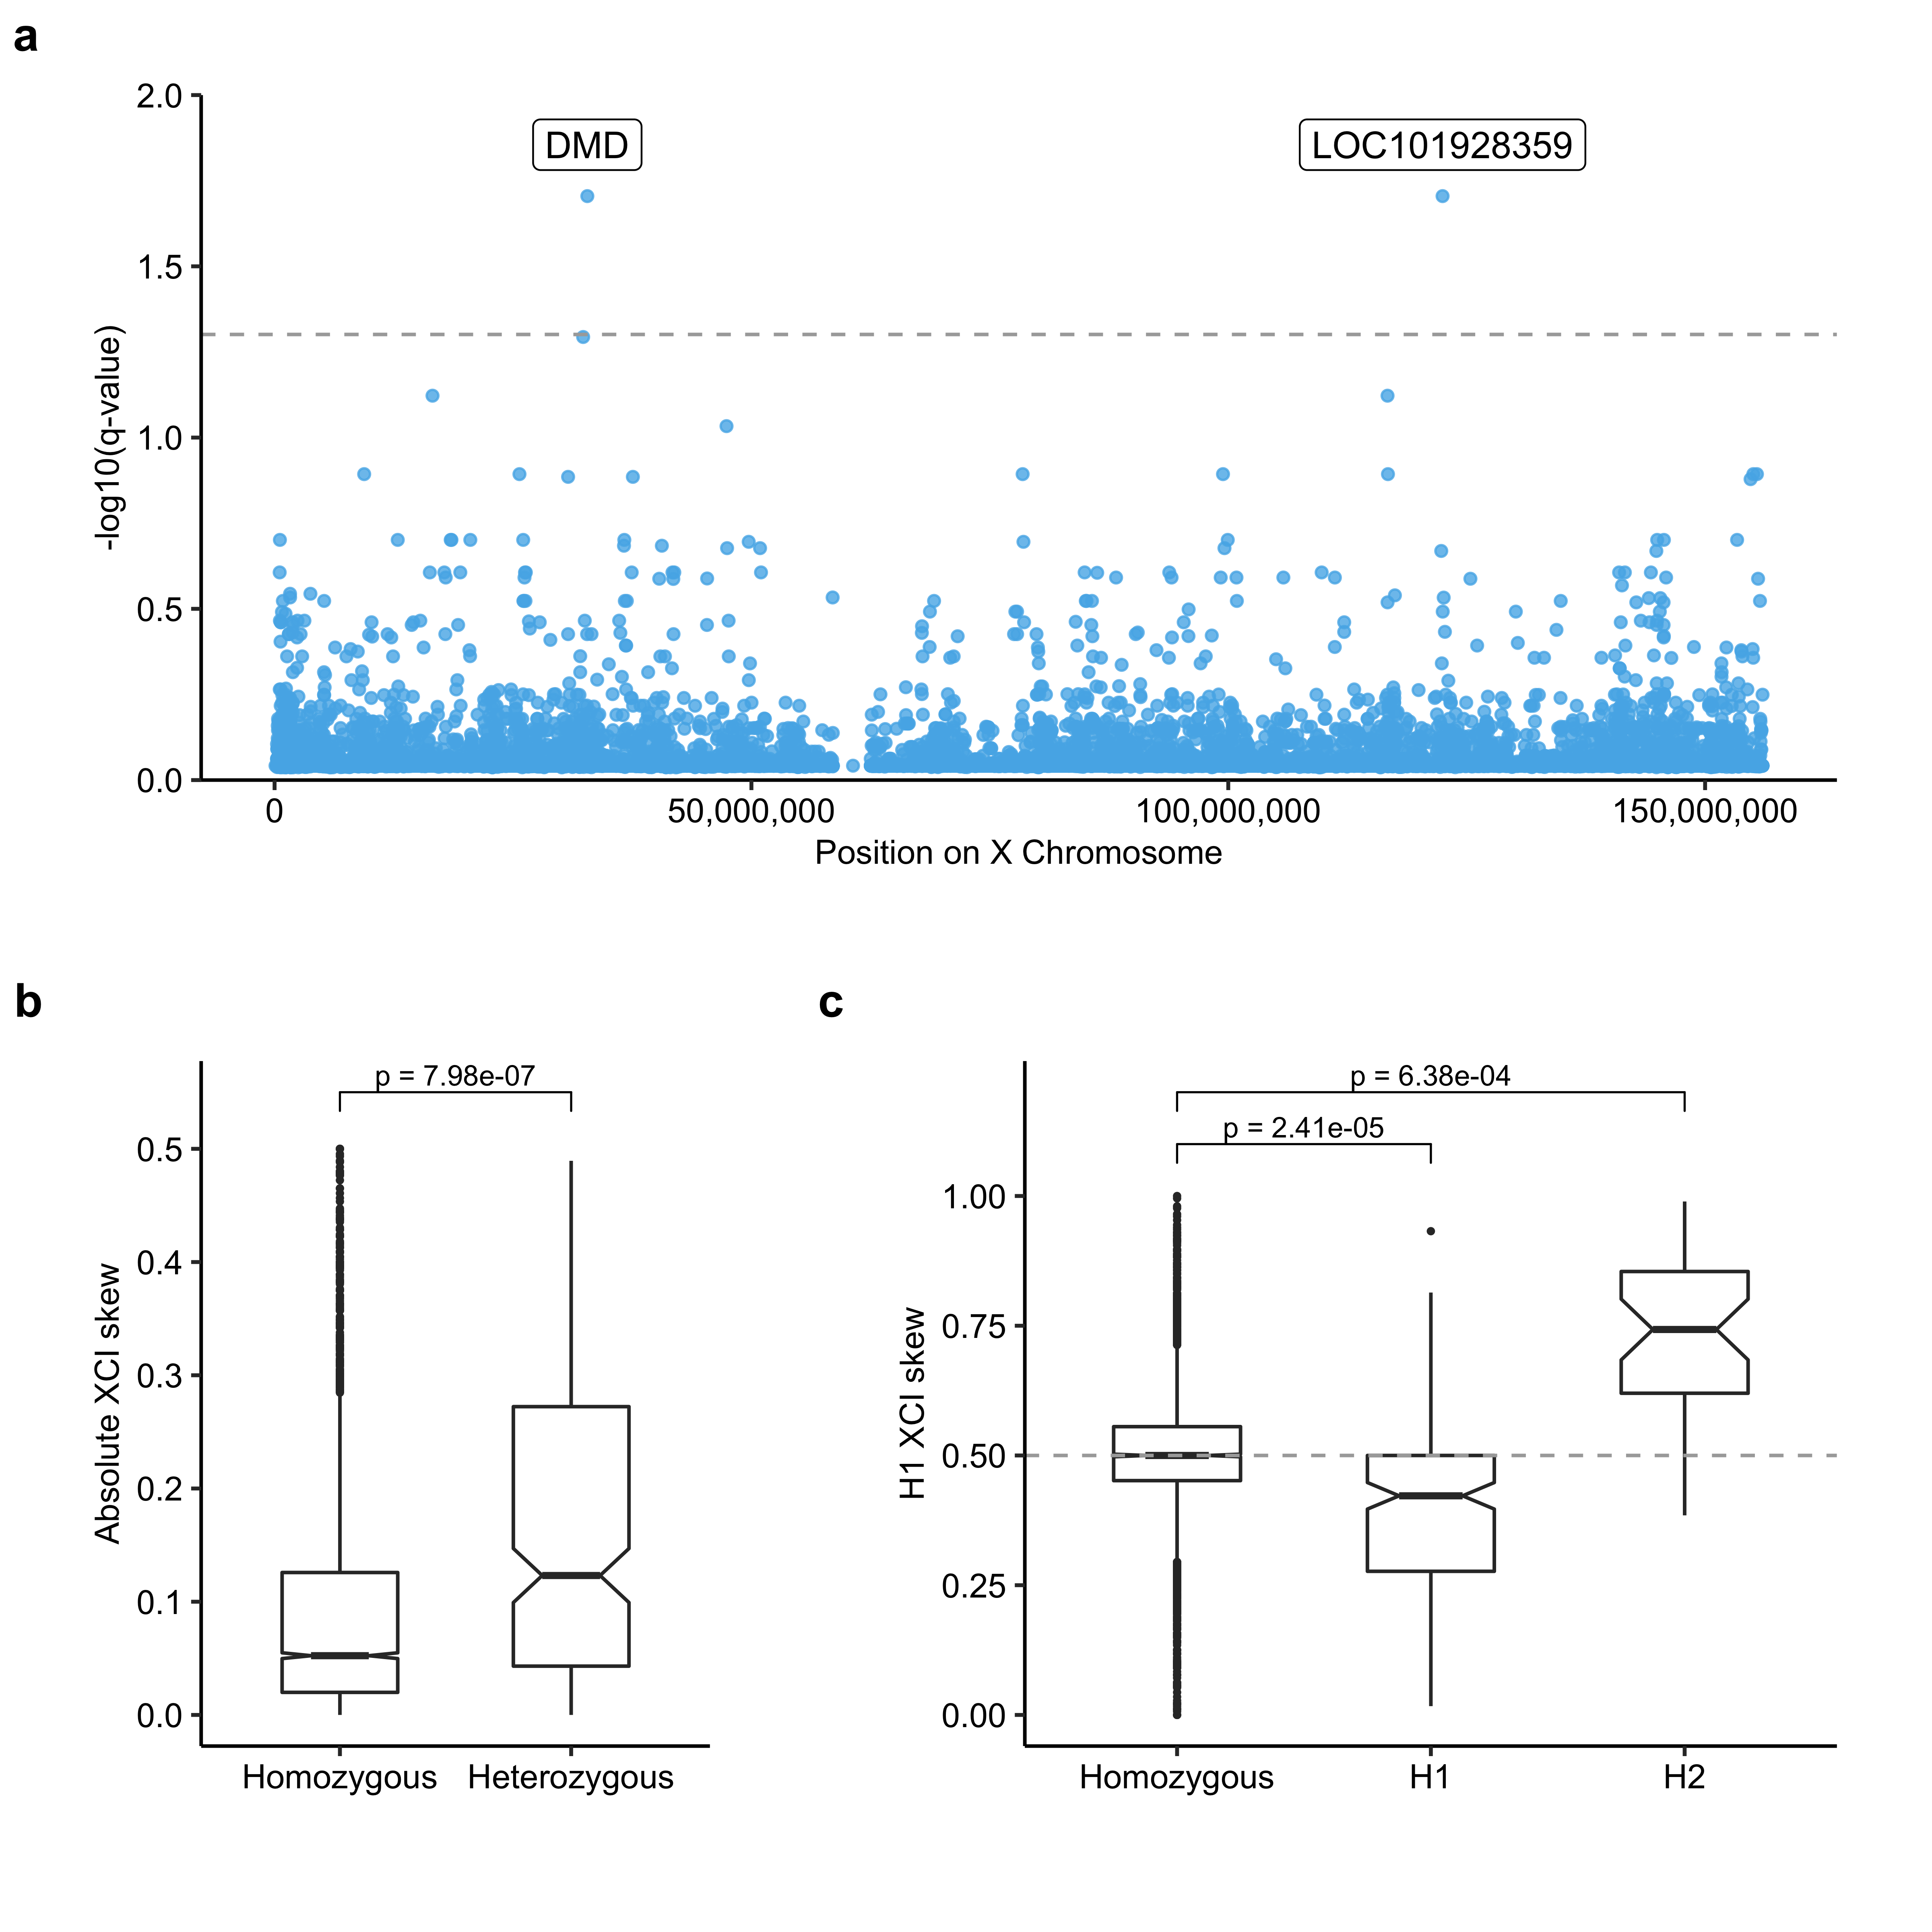
\includegraphics[width=0.75\textwidth]{chapter4/Figures/Figure_3.png}
    \caption{
        Associating specific variation on the X chromosome with inactivation skew. 
        \textbf{a}, Manhattan plot of -log10(q-values) generated from a linear mixed model associating absolute XCI skew with heterozygous status, accounting for age as well as individual and tissue groupings of samples. A one-sided test was performed under the hypothesis that heterozygous status increases absolute skew. Dotted horizontal line indicates local false discovery rate of 0.05. 
        \textbf{b}, Boxplot of absolute XCI skew in samples that are homozygous  (n = 4,232) or heterozygous (n = 230) for the DMD variant (rs141680486). Indicated p-value is from the model described above.
        \textbf{c}, Boxplot of skewing toward haplotype 1 (H1), where the grouping on the x-axis describes individuals without the DMD variant (Homozygous, n = 4,232), with the variant on haplotype 1 (H1, n = 190), and with the variant on haplotype 2 (H2, n = 40). Indicated p-values are from the model described above but with a two-sided test, since we do not assume the direction of skewing associated with a specific variant.}
    \label{fig:fig4.3}
\end{figure}
\begin{figure}[ht!]
    \centering
    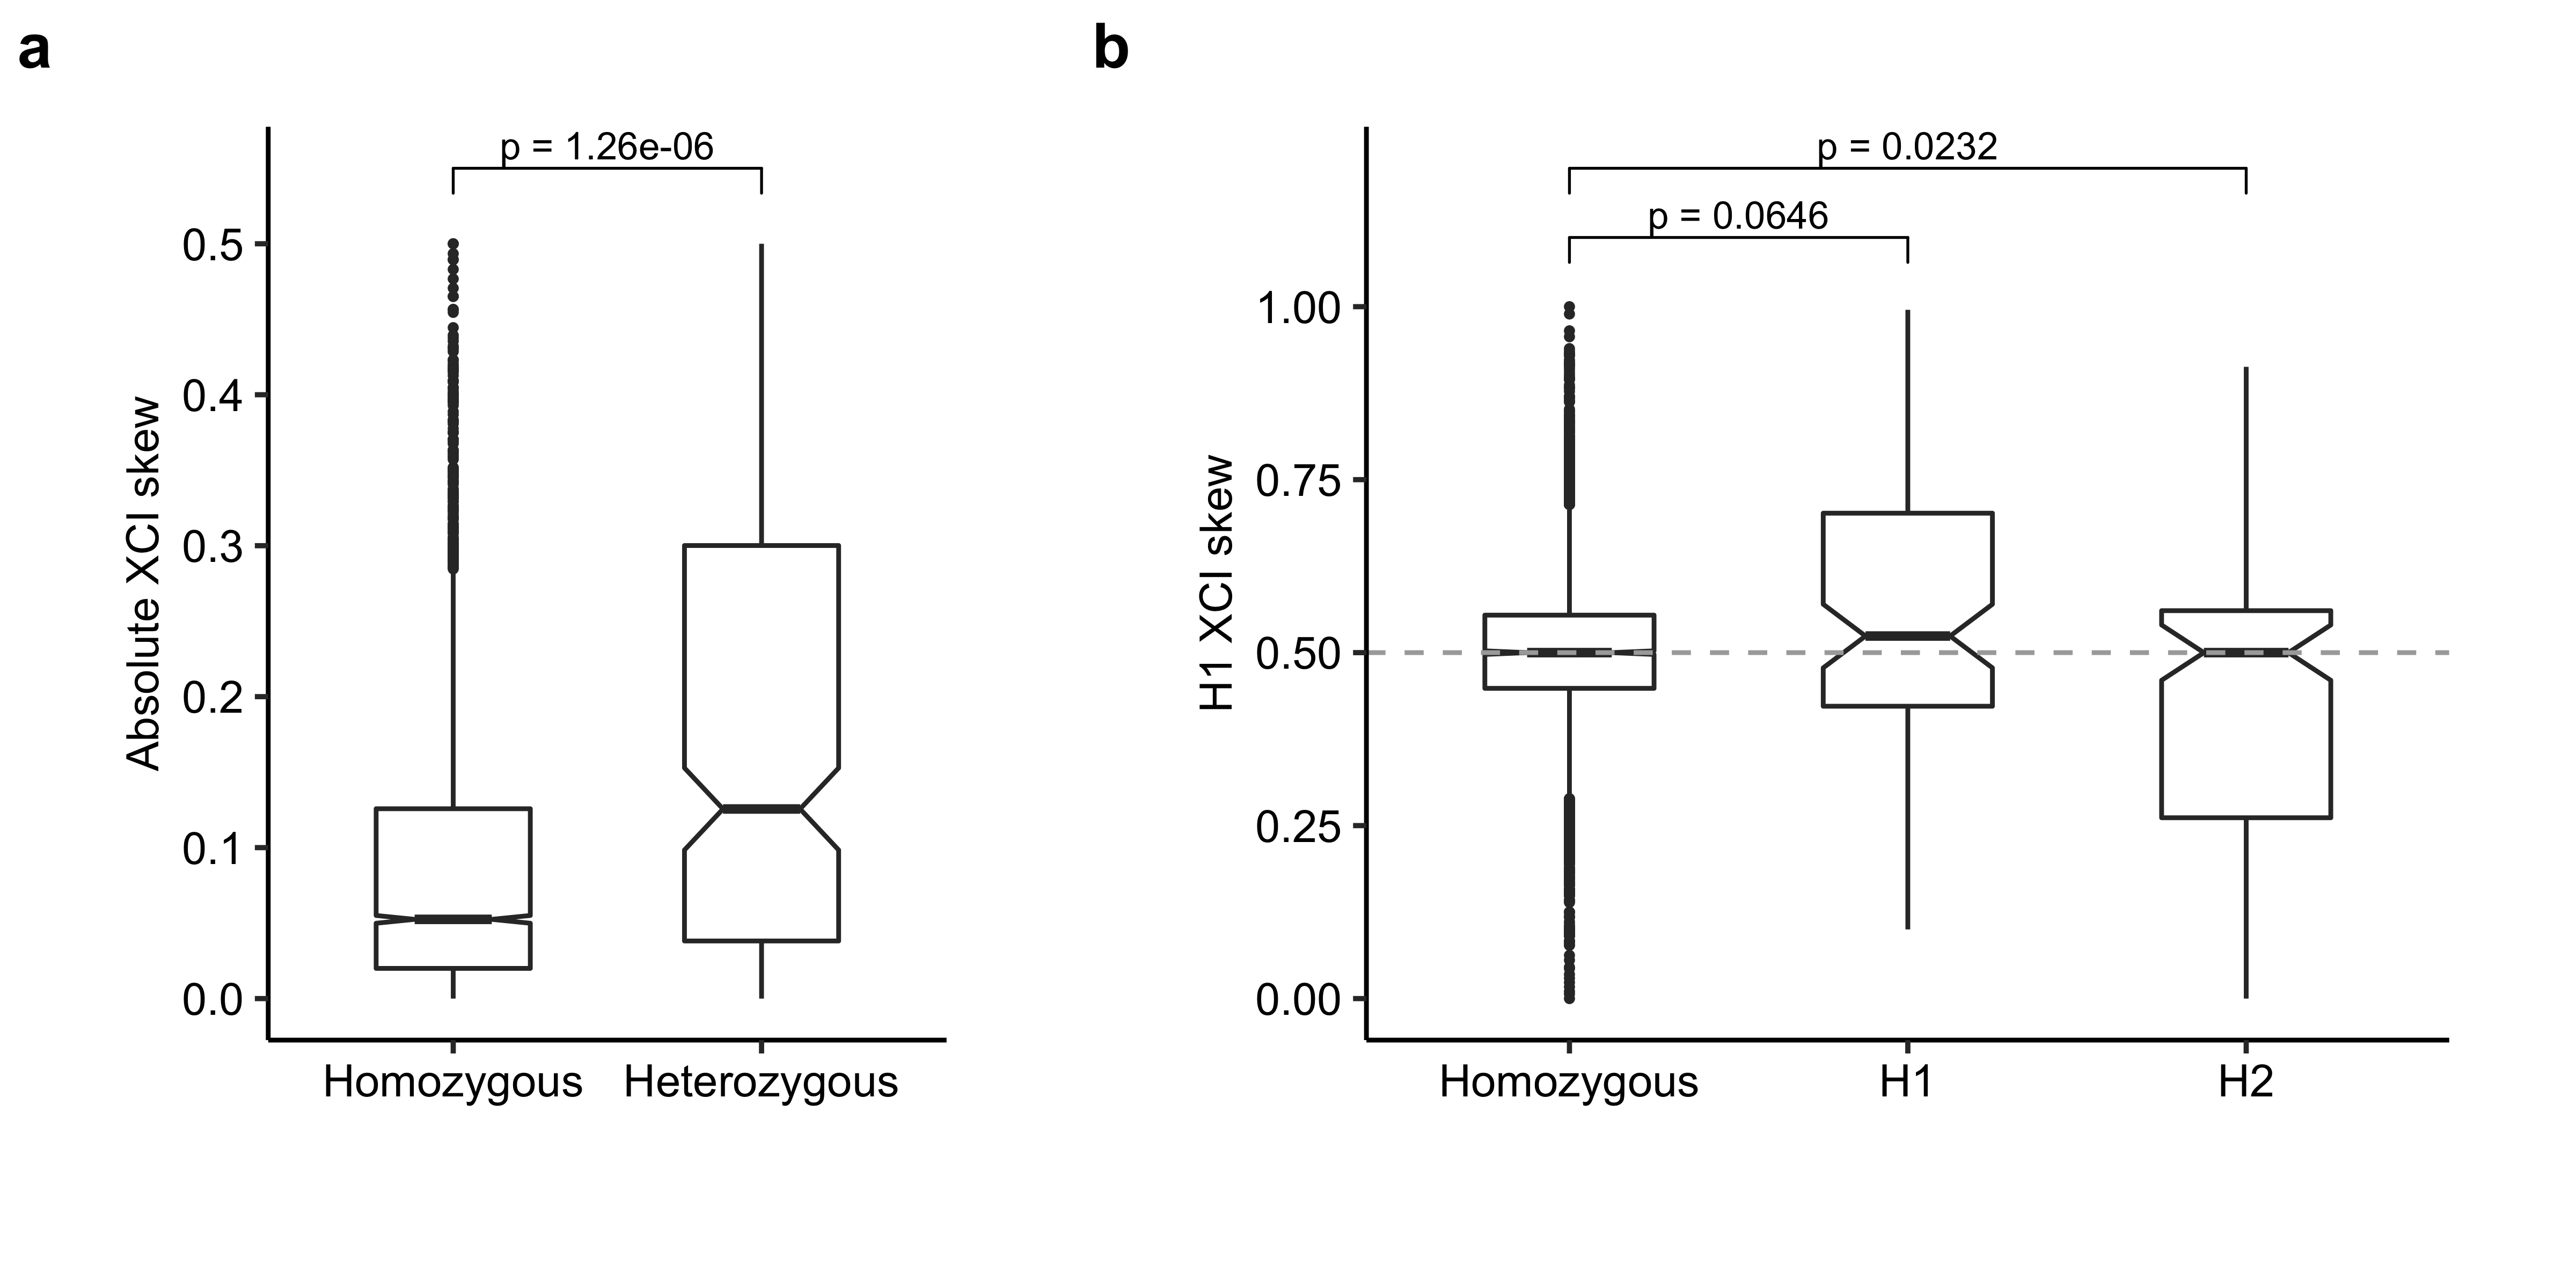
\includegraphics[width=0.9\textwidth]{chapter4/Figures/Supplementary_Figure_4.png}
    \caption{
        Association of LOC101928359 variant (rs73227260) variants with XCI skew. Indicated p-values are from a linear mixed model accounting for individual and tissue of origin.
        \textbf{a}, Boxplot of absolute XCI skew in homozygous samples (n = 4,230) and heterozygous samples (n = 232). Indicated p-value is from a one-sided t-test.
        \textbf{b}, Boxplot of skewing toward haplotype 1 (H1), where the grouping on the x-axis describes individuals without the LOC variant (Homozygous, n = 4,230), with the variant on haplotype 1 (H1, n = 92), and with the variant on haplotype 2 (H2, n = 140). Indicated p-values are from two-sided t-test.  
    }
    \label{fig:supp_fig4.4}
\end{figure}
\begin{table}[ht]
\scriptsize
\caption{Top 10 variants associated with absolute skewing in XCI}
\centering
\begin{tabular}{lllllll}
  \hline
Locus & SNP & Position & Alleles & AF & $\beta$ (s.e.) & $P_{\text{one-sided}}$ \\ 
  \hline
  DMD & rs141680486 & 32794582 & C/G & 0.0179 & 0.0203 (0.0041) & 7.978e-07 \\ 
  LOC101928359 & rs73227260 & 122471389 & C/T & 0.0203 & 0.0199 (0.0041) & 1.265e-06 \\ 
  DMD & rs144615018 & 32355895 & C/G & 0.0328 & 0.0175 (0.0039) & 4.891e-06 \\ 
  None & rs140456300 & 116700067 & A/T & 0.0316 & 0.0157 (0.0036) & 9.868e-06 \\ 
  None & rs113265091 & 16560720 & T/C & 0.0185 & 0.0177 (0.0041) & 1.21e-05 \\ 
  ZNF157 & rs140428205 & 47388509 & G/A & 0.0215 & 0.0174 (0.0041) & 1.782e-05 \\ 
  None & rs60102760 & 9394922 & T/G & 0.0263 & 0.0168 (0.0041) & 2.917e-05 \\ 
  FUNDC2 & rs782070621 & 155057031 & T/G & 0.0369 & 0.0169 (0.0042) & 3.742e-05 \\ 
  None & rs139564137 & 155434572 & C/T & 0.0358 & 0.0169 (0.0042) & 3.742e-05 \\ 
  None & rs6623805 & 78439230 & A/T & 0.9475 & 0.0159 (0.004) & 4.263e-05 \\ 
   \hline
\end{tabular}
\label{table:table4.3}
\end{table}

\section{Discussion}

These analyses support the hypothesis that differences in genetic variation on the maternal and paternal X chromosomes influences skewed inactivation through selection \cite{Brown1999-dc,Migeon1998-gc}. Specifically, these results demonstrate a significant association between higher CADD scores of a haplotype and estimated skewing away from this haplotype. Furthermore, we showed that higher polygenic scores related to proliferation, specifically red blood cell and basophil counts, tend to be associated with skewing towards the haplotype. These results imply that skewing in X inactivation may arise from higher proliferation or reduced deleteriousness of cells with one haplotype activated compared to the other subpopulation. We also identified common variation within specific loci on the X chromosome, such as the dystrophin gene, associated with XCI skew that may also contribute to these differences in proliferation or deleteriousness.

Several confounding factors could influence the results of this study. First, haplotype estimation by phasing algorithms may be inaccurate. Phasing errors would reduce the power of these analyses, since genetic scores may include variants from both haplotypes. In our analyses, we observed phase switches in EBV-transformed lymphocyte samples with extreme XCI skewing that suggests some phasing errors had occurred. Second, mapping biases may cause artificially higher observed expression of reference alleles compared to alternate alleles. This issue is addressed by the WASP filtering \cite{Van_de_Geijn2015-oy} used in the alignment of RNA-seq reads. Third, differences in eQTL effects across haplotypes may lead to skewed expression in RNA-seq experiments that may be incorrectly attributed to skewed XCI. We consider this source of confounding by taking the median of expression skew measured across heterozygous sites in 117 fully inactivated genes and by testing whether our features of interest are significant in the non-acrocentric autosomes or as eQTLs in the male samples. These issues could be circumvented with sufficiently large single-cell RNA-seq datasets. Haplotype phasing, as well as inactivation status, could be estimated within each cell individually and XCI skew could be calculated by simply counting cells. Furthermore, these data would allow cell-type-specific analysis of the relationship between genetics and skewed XCI.  

The influence of genetics on XCI skewing across the general female population highlights interesting mechanisms that should be further explored. For example, the effect of a specific variant on a complex phenotype may be dampened or amplified depending on the haplotype that carries it in females. For example, if an individual homozygous for a disease-related variant carries it on a haplotype with reduced proliferation, its effect may be dampened since a majority of cells will be expressing the wild-type variant. Epistatic effects and reduced penetrance due to allele-specific expression has been previously reported in the context of allele-specific gene regulation \cite{Castel2018-wo,Lappalainen2011-mu}. Here, these effects would arise from skewed X inactivation across a tissue rather than skewed expression within individual cells. This effect on penetrance has been described in the context of X-linked disorders, where skewed inactivation blurs the distinction of dominant and recessive traits across males and females \cite{Dobyns2004-ac}. The results shown here imply that selective pressures on genetic differences across the female population can influence skewing and consequently influence the penetrance of variation across the X chromosome.
